%Auteurs : Nicolas Englebert
\documentclass[british,french,11pt, a4paper, openany]{book}

% Règles de bonne pratiques :
% https://fr.wikibooks.org/wiki/LaTeX/Gestion_des_gros_documents
\usepackage{../../Builder/preambule}
% %%%%%%%%%%%%%%%%
%%% Packages %%%
%%%%%%%%%%%%%%%%

%%% Compatibilité %%%
\begingroup\expandafter\expandafter\expandafter\endgroup
\expandafter\ifx\csname IncludeInRelease\endcsname\relax
\usepackage{fixltx2e}
\fi 					% Si version LaTeX < 2015, inclut un fix.

%%% Général %%%
\usepackage[utf8]{inputenc}
\usepackage{babel}
\usepackage{lmodern}
\usepackage[T1]{fontenc}
\addto\extrasfrench{\sisetup{locale = FR,detect-all}} % Switch siunitx en fonction de la langue babel :)
\addto\extrasbritish{\sisetup{locale = UK,detect-all}}
\usepackage{courier}
\usepackage{graphicx}
%\usepackage{cancel}

%%% Tableau %%%
%\usepackage{tabularx} %Permet d'auto dimensionner les tableaux



%%% Bibliographie %%%
%\usepackage[style=alphabetic,backend=biber]{biblatex}
\usepackage[autostyle]{csquotes}
%\DeclareNameAlias{sortname}{last-first}
%\DeclareFieldFormat{url}{\space\url{#1}}
%\DeclareNameAlias{labelname}{last-first}
%\addbibresource{sample.bib}


%%% Graphiques %%%
%\usepackage{tikz}
%\usepackage{pgfplots}
%\usepackage{circuitikz}

%%% Mise en page %%%
\usepackage{mathtools}
\usepackage{amssymb}
\usepackage{bbm}
\usepackage{amsthm}
%\usepackage[tt]{titlepic}% Centre le titre
%\usepackage{fancyhdr}   % Permet de modifier l'entête & footer
\usepackage{caption}     % Permet d'ajouter des légendes en images sans les mettre en float + dans la marge + ref vers le haut de l'envirronement
\usepackage{wrapfig}
\usepackage{fullpage}
%\usepackage{multicol}   % pour les liste sur plusieurs colonnes
%\usepackage{subfigure}  % alligne deux images cote a cote
\usepackage{float}      %permet de mettre du texte entre les figures grace a [H]. Génial! 
\usepackage{eso-pic}    % Fond d'écran page de garde
\usepackage{adjustbox}  % Empêche les box de sortir de la page


%%% Math %%%
%\usepackage{delarray} % Belles matrices
\usepackage{siunitx}


%%% Codes %%%
%\usepackage{listings}
%\usepackage[final]{pdfpages} %% Inclusion fichier pdf

%% Reference
\usepackage{hyperref}
%\renewcommand*{\figureautorefname}{fig.}
%\def\appendixautorefname{annexe}
%\def\tableautorefname{tab.}
%\renewcommand*{\chapterautorefname}{ch.}
%\newcommand{\subfigureautorefname}{\figureautorefname}



%%%%%%%%%%%%%%%%%
%%% Commandes %%%
%%%%%%%%%%%%%%%%%

%%% Physique %%%
\newcommand{\cst}{\text{cst}}
\newcommand{\D}{\partial}
\newcommand{\E}{\vec E}
\newcommand{\B}{\vec B}
\newcommand{\F}{\vec F}
\newcommand{\modu}[1]{|$#1$|}

%%% Math %%%
\newcommand{\oiint}{\int\!\!\!\!\!\!\! \:\!\subset\!\!\supset\!\!\!\!\!\!\!\int}
\newcommand{\rot}{\operatorname{\vec{rot}}}
\newcommand{\divv}{\operatorname{div}}
\newcommand{\phas}[1]{\underline{#1}}
\newcommand{\RE}{\text{Re}}
\newcommand{\ft}{\overset{\mathcal{F}}{\longleftrightarrow}}
\newcommand{\lt}{\overset{\mathcal{L}}{\longleftrightarrow}}
\newcommand{\DS}{\displaystyle}
\newcommand{\Tr}{\operatorname{Tr}}



%% Box
\shorthandon{:}
\newcommand{\theor}[1]{\adjustbox{minipage=\linewidth-2\fboxsep-2\fboxrule,fbox}{\textsc{\iflanguage{british}{Theorem}{Théorème}: }#1}}
\newcommand{\defi}[1]{\adjustbox{minipage=\linewidth-2\fboxsep-2\fboxrule,fbox}{\textsc{\iflanguage{british}{Definition}{Définition}: }#1}}
\newcommand{\lemme}[1]{\adjustbox{minipage=\linewidth-2\fboxsep-2\fboxrule,fbox}{\textsc{\iflanguage{british}{Lemma}{Lemme}: }#1}}
\newcommand{\prop}[1]{\adjustbox{minipage=\linewidth-2\fboxsep-2\fboxrule,fbox}{\textsc{\iflanguage{british}{Property}{Propriété}}\\ #1}}
\newcommand{\proposition}[1]{\adjustbox{minipage=\linewidth-2\fboxsep-2\fboxrule,fbox}{\textsc{Proposition}\\#1}}
\newcommand{\cadre}[1]{\adjustbox{minipage=\linewidth-2\fboxsep-2\fboxrule,fbox}{#1}}
\newcommand{\retenir}[1]{\adjustbox{minipage=\linewidth-2\fboxsep-2\fboxrule,fbox}{\textbf{\textit{\textsc{\iflanguage{british}{To remember}{À retenir}}: }}#1}}

\newcommand{\corollaire}[1]{\bigbreak\begin{tabular}{||c}
	\begin{minipage}{\textwidth}
		\textsc{\iflanguage{british}{Corollary}{Corollaire}: } \textit{#1}
	\end{minipage}
	\end{tabular}}
\newcommand{\exemple}[1]{\bigbreak\begin{tabular}{|c}
	\begin{minipage}{\textwidth}
		\textsc{\iflanguage{british}{Example}{Exemple}: } #1
	\end{minipage}%
	\end{tabular}}%
\shorthandoff{:}
    

%\pagestyle{headings} % Titre du ch et numéro page dans l'entete
%\renewcommand{\proofname}{Démonstration}
%\addto\captionsfrench{\def\tablename{Tableau}}


%%% Background %%%
\newcommand\BackgroundPic{%
	\put(0,0){%
		\parbox[b][\paperheight]{\paperwidth}{%
			\vfill
			\centering
			\includegraphics[width=\paperwidth,height=\paperheight,%
			keepaspectratio]{../../Builder/ulb.jpg}%
			\vfill
}}}

%%% Annexes Cedu %%%
%\usepackage{calrsfs}
%\DeclareMathAlphabet{\pazocal}{OMS}{zplm}{m}{n}
\usepackage{fourier-orns}

\setlength{\parindent}{0pt} 

%%% Attributs %%%
\newcommand*{\NomduCours}[2]{\def\cours{#1}\def\memo{#2}}
\newcommand*{\annee}[2]{\def\adebut{#1}\def\afin{#2}}

\newcounter{auteurcnt}
\newcommand\addauteur[2]{%
	\stepcounter{auteurcnt}%
	\csdef{auteur\theauteurcnt}{\mbox{#1~\textsc{#2}}}}
\newcommand\getauteur[1]{%
	\csuse{auteur#1}}

\newcounter{illustrateurcnt}
\newcommand\addillustrateur[2]{%
	\stepcounter{illustrateurcnt}%
	\csdef{illustrateur\theillustrateurcnt}{\mbox{#1~\textsc{#2}}}}
\newcommand\getillustrateur[1]{%
	\csuse{illustrateur#1}}

\newcounter{rappeltheocnt}
\newcommand\addrappeltheo[2]{%
	\stepcounter{rappeltheocnt}%
	\csdef{rappeltheo\therappeltheocnt}{\mbox{#1~\textsc{#2}}}}
\newcommand\getrappeltheo[1]{%
	\csuse{rappeltheo#1}}

\newcounter{professeurcnt}
\newcommand\addprofesseur[2]{%
	\stepcounter{professeurcnt}%
	\csdef{professeur\theprofesseurcnt}{\mbox{#1~\textsc{#2}}}}
\newcommand\getprofesseur[1]{%
	\csuse{professeur#1}}

\newcounter{iter}

% Attributs
\NomduCours{Chimie générale}{CHIM-H-100}
\addauteur{Nicolas}{Englebert}
\addprofesseur{Philippe}{Bogaerts}
\annee{2013}{2014}


% Document
\begin{document}
\def\equationautorefname~#1\null{%
	(#1)\null
}
%%%%%%%%%%%%%%%%%
% Préliminaires %
%%%%%%%%%%%%%%%%%
\frontmatter
\AddToShipoutPicture*{\BackgroundPic}

\begin{titlepage}
	\begin{center}	
			
		\newcommand{\HRule}{\rule{\linewidth}{0.5mm}}   			            %Titre en gros
		\includegraphics[width=0.55\textwidth]{../../Builder/titlepage/logo.pdf}~\\[1cm]				%Logo
			
			\textsc{\LARGE Université Libre de Bruxelles}\\[1.5cm]
			\textsc{\Large \iflanguage{british}{Summary}{Synthèse}}\\[0.5cm]
			
			\HRule \\[0.4cm]
			{ \huge \bfseries \cours \ \\\memo \\[0.4cm] }
			
			
			\HRule \\[1.5cm]
			\begin{minipage}[t]{0.6\textwidth}
				\begin{flushleft}%\large
					\emph{\iflanguage{british}{Author}{Auteur}\ifnum\theauteurcnt>1 s\fi:}\\
					\whileboolexpr
					{ test {\ifnumcomp{\value{iter}}{<}{\theauteurcnt}} }%
					{\stepcounter{iter}\getauteur{\theiter}\\}
					\setcounter{iter}{0}%
					\ifnum\theillustrateurcnt>0%
					\ \\
					\emph{Illustrations:}\\
					\whileboolexpr
					{ test {\ifnumcomp{\value{iter}}{<}{\theillustrateurcnt}} }%
					{\stepcounter{iter}\getillustrateur{\theiter}\\}%
					\setcounter{iter}{0}%
					\fi%
					\ifnum\therappeltheocnt>0%
					\ \\
					\emph{\iflanguage{british}{Reminders}{Rappels théoriques}:}\\
					\whileboolexpr
					{ test {\ifnumcomp{\value{iter}}{<}{\therappeltheocnt}} }%
					{\stepcounter{iter}\getrappeltheo{\theiter}\\}%
					\setcounter{iter}{0}%
					\fi%
				\end{flushleft}
			\end{minipage}%
			\begin{minipage}[t]{0.25\textwidth}
				%\begin{flushright}
				%\large
				\emph{\iflanguage{british}{Professor}{Professeur}\ifnum\theprofesseurcnt>1 s\fi:}
				\whileboolexpr
				{ test {\ifnumcomp{\value{iter}}{<}{\theprofesseurcnt}} }%
				{\\ \stepcounter{iter}\getprofesseur{\theiter}}%
				\setcounter{iter}{0}%
				%\end{flushright}
			\end{minipage}
			
			\vfill
			
			% Bottom of the page
			{\large \iflanguage{british}{Year}{Année} \adebut~-~\afin}
			
		\end{center}
	\end{titlepage}

\ \\[2cm]
{\Huge \bfseries Appel à contribution}\\[5mm]
\subsection*{Synthèse Open Source}
\begin{wrapfigure}[5]{l}{4.5cm}
	\includegraphics[scale=0.5]{../../Builder/git.png}
\end{wrapfigure}
Ce document est grandement inspiré de l’excellent cours donné 
par \ifnum\theprofesseurcnt=1 \getprofesseur{1} \else\whileboolexpr
{ test {\ifnumcomp{\value{iter}}{<}{\theprofesseurcnt-2}} }%
{\stepcounter{iter}\getprofesseur{\theiter}, }%
\stepcounter{iter}\getprofesseur{\theiter} et \stepcounter{iter}\getprofesseur{\theiter} \fi%
 à l’EPB (École Polytechnique de Bruxelles), faculté de l’ULB (Université 
Libre de Bruxelles). Il est écrit par les auteurs susnommés avec l’aide de tous les autres étudiants 
et votre aide est la bienvenue ! En effet, il y a toujours moyen de l’améliorer surtout que si le 
cours change, la synthèse doit être changée en conséquence. On peut retrouver le code source à l’adresse 
suivante
\begin{center}
	\url{https://github.com/nenglebert/Syntheses}
\end{center}\bigskip
Pour contribuer à cette synthèse, il vous suffira de créer un compte sur \textit{Github.com}. De
légères modifications (petites coquilles, orthographe, ...) peuvent directement être faites sur le
site ! Vous avez vu une petite faute ? Si oui, la corriger de cette façon ne prendra que quelques 
secondes, une bonne raison de le faire ! \bigskip

Pour de plus longues modifications, il est intéressant de disposer des fichiers : il vous 
faudra pour cela installer \LaTeX, mais aussi \textit{git}. Si cela pose problème, nous sommes 
évidemment ouverts à des contributeurs envoyant leur changement par mail ou n’importe quel autre 
moyen.\bigskip

Le lien donné ci-dessus contient aussi un \texttt{README} contenant de plus amples informations, 
vous êtes invités à le lire si vous voulez faire avancer ce projet ! 

\subsection*{Licence Creative Commons}
\begin{wrapfigure}[3]{r}{2.8cm}
	\vspace{-5mm}
	\includegraphics[scale=0.17]{../../Builder/CC}
\end{wrapfigure}
Le contenu de ce document est sous la licence Creative Commons : \textit{Attribution-NonCommercial-ShareAlike 
4.0 International (CC BY-NC-SA 4.0)}. Celle-ci vous autorise à l'exploiter pleinement, compte-
tenu de trois choses :
\begin{enumerate}
	\item \textit{Attribution} ; si vous utilisez/modifiez ce document vous devez signaler le(s) nom(s)
	      de(s) auteur(s).
	\item \textit{Non Commercial} ; interdiction de tirer un profit commercial de l’œuvre sans 
	      autorisation de l'auteur 
	\item \textit{Share alike} ;  partage de l’œuvre, avec obligation de rediffuser selon la même 
	      licence ou une licence similaire
\end{enumerate}
Si vous voulez en savoir plus sur cette licence :
\begin{center}
	\url{http://creativecommons.org/licenses/by-nc-sa/4.0/}
\end{center}

\begin{flushright}
	\textbf{Merci ! }
\end{flushright}
\tableofcontents
%Si abstract, \input ici

%%%%%%%%%%%%%%%%%%%%%
% Contenu principal %
%%%%%%%%%%%%%%%%%%%%%
\mainmatter
\chapter{Équilibre chimique}
\section{Etat d'équilibre}
Être à l'équilibre ne signifie pas qu'il n'y a plus de transformations chimiques. Il y a équilibre lorsque la vitesse de réaction directe vaut la vitesse de la réaction inverse.

\section{Constante d'équilibre}
La loi de Guldberg et Waage est totalement empirique : \textit{Loi d'action de masse}. Elle permet de reproduire les "choses" observées.\\
Les unités de $K$ dépendent de la réaction, mais elle sont facultatives. Cette constante dépend de la stœchiométrie.\\

Cette loi est appliquabl à des mélanges de gaz (pas à pression élevée) et à des solutions liquides diluées. Pour \textbf{une} température donnée, il existe \textsc{une et une seule} constante d'équilibre $K$. Mais pour une température donnée il existe une infinité de \textbf{position d'équilibre}. Les concentrations ne sont que des contraintes.

\section{Constante d'équilibre en fonction des pressions}
Une seule relation à retenir ! On peut la retrouver en partant de $pV = nRT$.
$$K_p = K(RN)^{\Delta n}$$

\section{Équilibre hétérogène}
Si on se trouve dans un cas avec plus d'une phase, on est dans un équilibre hétérogène. La position d'équilibre hétérogène est \textbf{indépendante} de la quantité de solide ou liquide \textit{purs}.

\section{Application de la constante d'équilibre}
La constante informe de la tendance naturelle de la réaction à se produire mais ne dit \textbf{rien} sur sa vitesse.\\
Plusieurs cas possibles :
\begin{enumerate}
	\item $K >> 1$ : Équilibre fortement déplacé à droite. A l'équilibre, il y a essentiellement des produits
	\item $K << 1$ : Équilibre fortement déplacé à gauche. A l'équilibre, il y a essentiellement des réactifs.
\end{enumerate}
On peut définir le sens d'une réaction avec le quotient réactionnel $Q$. Si $Q > K$ c'est qu'il y a trop de produit, l'équilibre se déplacera vers la gauche.

\section{Résolution de problèmes d'équilibres}
Pas de points théoriques, partie intégralement pratique (\textit{cf. TP}).

\section{Principe de le Chatelier}
Ici, on parle bien de l'équilibre et pas de la constante. Le principe est le suivant : 
\begin{center}
	\textit{Quand une action extérieure modifie un état d'équilibre, le système réagit de façon à s'opposer à cette action extérieure}.
\end{center}
Il y a trois facteurs qui influence l'équilibre (\textbf{pas} le constante, sauf la 3 !)
\begin{enumerate}
	\item La concentration
	\item La pression
	\item La température
\end{enumerate}
L'ajout d'un solide ou liquide pur n'a aucune influence sur la position d'équilibre. De plus ajouter un gaz inerte n'a aucune influence sur la position d'équilibre mais augmente la pression totale (donc influe sur les pressions partielles).

\newpage
\chapter{Réactions acide-base}
\section{Nature des acides et des bases}
Selon Arrhénius : 
\begin{description}
	\item[Acide] Substance qui produit des ions $H^+$ en solution aqueuse
	\item[Base] Substance qui produit des ions $PH^-$ en solution aqueuse
\end{description}
\ \\

Selon Bronsted-Lowry 
\begin{description}
	\item[Acide] Donneur de protons $H^+$
	\item[Base] Accepteur de protons $H^+$
\end{description}

Quand plusieurs base sont mis ensemble, il va y avoir une "compétition" pour savoir lequel mérite d'avoir un beau petit $H^+$.

\section{Force d'un acide}
Un acide fort se remarque par un $K_a$ très élevée et une dissociation quasi-complète.\\

Un \textit{amphotère} est une substance qui se comporte soit comme un acide, soit comme un base ; réaction d'auto-ionisation.

\section{Échelle de pH}
La variation d'une unité de pH correspond à une variation d'une puissance de 10 en $[H^+]$.

\section{Calcul du pH de solutions d'un acide fort}
Pas de points théoriques, partie intégralement pratique (\textit{cf. TP}).

\section{Bases}
Rien ne change, si ce n'est que le mot "acide" devient "base".

\section{Polyacides}
Il s'agit d'acides pouvant céder plus d'un protons. Bien souvent $K_{a1} >> K_{a2)}$ : Ceci est du au faut qu'après avoir arraché un $H^+$, ça devient plus compliquer d'en arracher un deuxième (c'est donc un moins bon acide).\\
On peut également expliquer ça en se disant que la charge négative d'un acide augmente, arracher une charge positive devient plus compliqué.

\section{Propriétés acide-base des sels}
Un sel est un composé ionique impliquant donc la présence d'ions en solution. Ils peuvent se comporter comme des acides, comme des bases ou simplement être spectateur. \\

\subsection{Sels produisant des solutions neutres}
Certains sels produisent donc des solutions neutres : La base conjuguée d'un acide fort est une base beaucoup plus faible que l'eau. Les ions ne se combinent donc pas aux $H^+$ et le sel n'a aucune influence sur le pH (par exemple, $Cl^-, NO_3^-, ...$).\\
Tout sel dont les cations proviennent d'une base forte et les anions d'un acide fort forment des solutions neutres.

\subsection{Sels produisant des solutions basiques}
La base conjugué d'un acide faible est une base plus forte que $H_2O$ : elle est capable de réagir avec les protons venant de l'eau et influencer le pH.\\
Les sels dont les cations proviennent d'une base forte et les anions d'un acide faible donnent des solutions basiques.

\subsection{Sels produisant des solutions acides}
Les sels dont les cations proviennent d'une base faible et les anions d'un acide fort donnent lieu à une solution basique. Les sels contenant un ion métallique fortement chargé pousse la solution à être acide. 

\subsection{Sels dont les deux ions peuvent modifier le pH}
Il a longuement insisté sur l'exemple du \textit{slide 44} (Lire aussi \textit{slide 45}).

\section{Influence de la structure sur les propriétés acide-base}
Facteurs influençant le caractère acide d'une molécule pour une liaison $H-X$ : 
\begin{enumerate}
	\item La force de la liaison (énergie nécessaire pour la briser)
	\item La polarité (quand les pôles sont confondus, la molécule est peu enclin à libérer ses précieux $H^+$).
\end{enumerate}
\ \\
Les oxacides comportent une liaison de type $H-O-X$ qui augmente l'acidité d'une solution grâce à la présence de $O$, très électronégatif (phénomène semblable au niveau des ions métalliques). De plus, l'électronégativité de $X$ joue aussi (si cette dernière est élevée, présence d'une liaison covalente forte), poussant à augmenter l'acidité de la molécule.

\section{Propriétés acide-base des oxydes}
Les oxydes covalents fortement une solution acide, c'est pourquoi on les appelle souvent \textit{oxydes acides}.\\
Par contre, les oxydes ioniques dissous dans l'eau forment une solution basique (l'ion $O^{2-}$ ayant une grande affinité pour $H^+$ (normal, il s'agit d'une base forte). 

\section{Acide et base de Lewis}
Théorie encore plus générale :
\begin{description}
	\item[Acide] Accepteur de doublets d'électrons
	\item[Base] Donneur de doublets d'électrons
\end{description}
Voici un petit tableau récapitulatif des trois théories : 
\begin{center}
	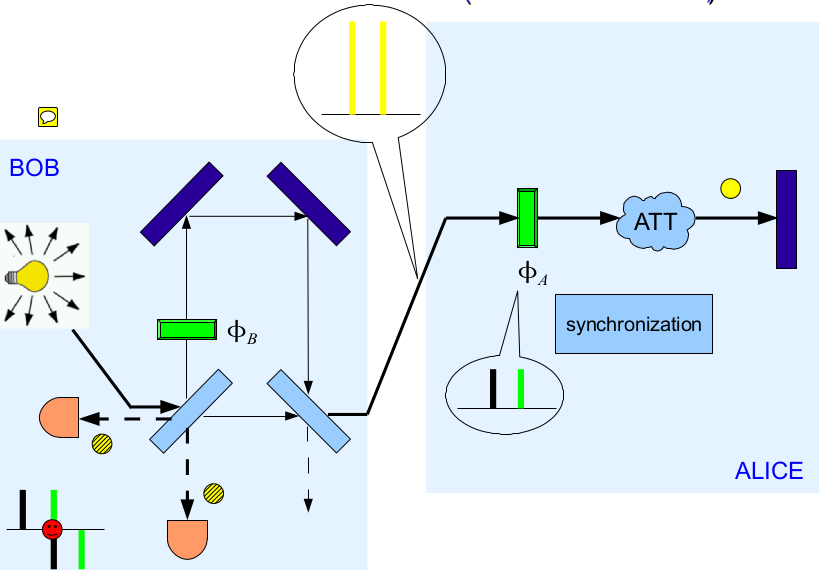
\includegraphics[scale=0.55]{image13.png}\\
\end{center}
Cette théorie englobe la théorie de Bronsted-Lowry mais l'inverse n'est pas vrai.

\section{Solutions d'acide ou de bases contenant un ion commun}
La présence d'un ions commun en solution déplace l'équilibre vers la gauche selon le principe de Le Chatelier rendant le pourcentage de dissociation plus faible. \\
Mettre du $NH_4^+$ en solution peut rendre la solution moins basique (Solution de $NH_3$ par exemple).

\section{Solutions tampons}
Il s'agit d'une solution dont le pH varie très peu après addition d'une petite quantité de $H^+$ ou $PH^-$.\\
Une solution tampon est constituée de (soit... ou soit): 
\begin{itemize}
	\item Un acide faible et son sel ($HF/NaF$)
	\item Une base faible et son sel ($NH_3/NH_4Cl$)
\end{itemize}
On peut utiliser la relation de Hendersen-Hasselbalch si l'on tient bien compte de l'hypothèse de faible dissociation (acide faible).

\section{Pouvoir tampon}
Il s'agit de la quantité de $H^+$ ou de $OH^-$ que l'on peut ajouter sans variation significative de pH. Celui-ci est déterminé par l'importance des concentrations acides et basiques. Plus ces \textbf{deux} concentrations sont élevées, plus le pouvoir tampon sera grand. 

\section{Titrage et courbes de titrage}
Le titrage est souvent utilisé pour déterminer la concentration d'une solution inconnue à l'aide de la solution titrante donc la concentration est connue.\\

Les deux dernières sections (\textit{Titrages et courbes de titrages} et \textit{Indicateurs colorés acide-base}) sont principalement constitués de graphiques, ... Je ne les inclus pas ici, mais ils semblent quand même important ! \\
\\
\\
\\
Comme c'est bête de gaspiller une page, je mets ici un dessin à colorier (sans dépasser!) pour que toi aussi, tu puisses être un vrai chimiste ! 

\begin{center}
	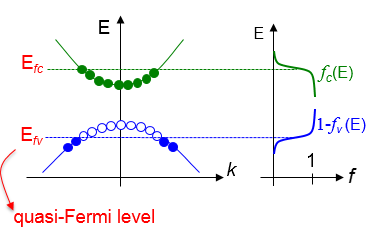
\includegraphics[scale=0.95]{image14.png}\\
\end{center}

\newpage
\chapter{Solubilité et réactions de précipitation}
\section{Réactions de précipitation et stœchiométrie de ces réactions}
Si un mélange donne lieu à une substance insoluble il y aura formation d'un précipité. Certaines règles sont à retenir par cœur :
\begin{center}
	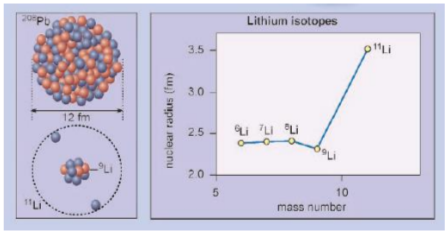
\includegraphics[scale=0.55]{image15.png}\\
\end{center}
\textit{NB :} S'il faut faire des calculs, il faut bien entendu se baser sur le réactif limitant.

\section{Équilibres ioniques et produit de solubilité}
Comme pour les constantes d'équilibre, on définit des produit de solubilité. La solubilité est le nombre de moles par litre de ... dissout.\\
Un solide pur n'intervient pas dans le $K_s$. Encore une fois, il n'y a qu'une seule constante d'équilibre pour une température donnée mais une infinité de position d'équilibre. La solubilité = position d'équilibre. \\

Le $K_p$ peut prédire la solubilité relative d'un groupe de sel si ceux-ci produisent le même nombre total d'ions en solutions ! Dans ce cas-la, le plus soluble sera celui ayant le $K_s$ le plus grand.\\

En cas d'ion commun, par le principe de Le Chatelier, la solubilité du sel en est diminuée. 

\section{Précipitation et analyse qualitative}
Comme pour le constante, on définit le \textbf{produit ionique $Q$} qui permet de prédire la formation d'un précipité.
\begin{itemize}
	\item $Q > K_s$ : Formation d'un précipité (diminution des $[\ ]_{eq}$)
	\item $Q < K_s$ : Pas de précipité
\end{itemize}
La précipitation sélective est utilisée pour séparer les ions métalliques. Elle consiste à utiliser un réactif dont l'anion formera un précipité avec un ou plusieurs des ions métalliques du mélange. 

\section{Équilibres des ions complexes}
Un ion complexe est une espèce chargée composée d'un ion métallique entouré de ligands (= base de Lewis (molécule ou ion possédant un doublet libre formant une liaison covalente avec l'ion métallique)).\\
Liaison ion-ligands se fait par étapes (un ligand à la fois) :
\begin{enumerate}
	\item Pour chaque étape, une constante d'équilibre
	\item Constante de formation ou de stabilité (cste d'eq. pour la formation d'un ion complexe (On la calcule comme pour un $K_a$))
\end{enumerate}

Le problème avec des ions complexe est qu'ils sont presque insoluble dans l'eau : problème au niveau de la dissolution de ces précipités pour séparer les ions qu'ils contiennent. On jouant sur les effets d'ions communs, on va pouvoir favoriser la solubilité.
\begin{center}
	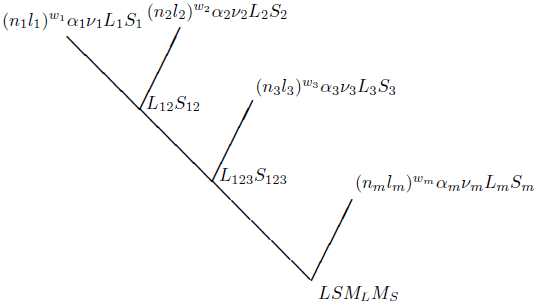
\includegraphics[scale=0.55]{image16.png}\\
\end{center}
\ \\
Méthodes pour dissoudre un solide ionique insoluble dans l'eau pure : 
\begin{enumerate}
	\item Acidification de la solution si l'anion du solide est une base efficace (n'irait pas avec $Cl^-$ qui est une base très faible et qui n'a pas d'affinité avec $H^+$)
	\item Ajout d'un ligand pour former un ion complexe stable avec le cation
	\item Combinaison des deux méthodes précédentes
	\item Augmentation de la température
\end{enumerate}

\newpage
\chapter{Réaction d'oxydo - réduction}
\subsection{Rappels}
L'oxydant est la substance qui accepte un ou plusieurs électrons. et le réducteur est la substance qui donne un ou plusieurs électrons.\\

L'oxydant est réduit et le réducteur est oxydé.

\section{Équilibrage des réactions d'oxydo-réduction}
\subsection{En solution acide}
Cette méthode est à suivre à la lettre et il n'y aura pas de soucis ! 
\begin{enumerate}
	\item Écriture des équations de demi-réactions d'oxydation et de réduction
	\item Équilibrage des demis réactions
	      \begin{enumerate}
	      	\item D'abord tout équilibrer sauf $H$ et $O$
	      	\item Équilibrage de $O$ à l'aide de $H_2O$
	      	\item Équilibrage de $H$ à l'aide de $H^+$
	      	\item Équilibrage des charges à l'aide d'électrons $e^-$
	      \end{enumerate}
	\item Égalisation du transfert d'électrons
	\item Addition des demi-réaction et annulation des espèces identiques
\end{enumerate}

\subsection{En solution basique}
On procède \textbf{exactement} de la même façon qu'en solution acide (on ajouté des $H^+$, ...). Puis arrivé à l'étape 4. il faut encore suivre trois étapes : \\
\begin{enumerate}
	\item Ajouter $OH^-$ dans les deux membres (Si trois à gauche, trois à droite) pour éliminer les $H^+$.
	\item Éliminer un maximum de $H_2O$ (formé par l'ajout d'$OH^-$) (simplification à gauche et à droite).
	\item Vérification des bilans de matière et de charge.
\end{enumerate}

\newpage
\chapter{Thermodynamique chimique}
La thermodynamique est la branche de la chimie physique qui étudie les transformations de l'énergie. L'énergie est la capacité à effectuer du travail.

\section{Premier principe}
Le premier principe met en avant la conservation de l'énergie. Avant tout, quelques définitions sont importantes : 
\begin{description}
	\item[Système] Partie de l'univers que l'on étudie
	\item[Milieu extérieur] Ce qui est à l'extérieur du systèpme, milieu dans lequel les expériences sont effectuées.
	\item[Système ouvert] Échange de matière et d'énergie possible avec le milieu extérieur
	\item[Système fermé] Pas d'échange avec le milieu extérieur (mais échange d'énergie possible)
	\item[Système isolé] Ni échange de matière ni échange d'énergie avec le milieu extérieur
	\item[Système adiabatique] Système thermiquement isolé de son milieu extérieur
\end{description}
\subsection{Travail et chaleur}
Il y a deux façon de modifier l'énergie d'un système fermé : sous forme de travail ou sous forme de chaleur.\\
Le travail est un transfert d'énergie qui opère un mouvement uniforme dans le milieu extérieur, ou l'utilise.\\
La chaleur est un transfert d'énergie qui opère un mouvement désordonné dans le milieu extérieur, ou l'utilise.

\subsection{La mesure du travail}
La définition du travail est une distance multiplié par une force opposée.
$$W = p_{ext}.\Delta V$$
Il est possible de calculer le travail maximum effectué par un gaz se dilatant de façon isotherme (car le système doit évoluer de façon réversible). Dans ce cas, le travail diminue au fur et à mesure que $V$ augmente (Boyle)
$$W = -nRT\ln\left(\frac{V_f}{V_i}\right)$$
où le - reflète le principe de l'énergie interne (on considère ici une expansion).

\subsection{L'énergie interne}
L'énergie interne est l'énergie transférée à un système (somme de toutes les $E_c$ et $E_p$). Sa mesure est impossible, mais les variations oui.
$$\Delta U = w + q$$
Si celle-ci est positive c'est que l'énergie interne augmente (on effectue un travail sur lui ou on lui administre de la chaleur).
\begin{center}
	\textit{Premier principe : L'énergie interne d'un système isolé est constante}
\end{center}

\subsection{Le premier principe}
Lors d'un transfert d'énergie à un système à volume constant, l'énergie interne augmente. L'expérience montre que 
$$\Delta T = \frac{q}{C}$$
où $C$ est la capacité calorifique qui dépend de la taille de l'échantillon. Elle est différente à volume ou à pression constante. Pour un gaz parfait :
$$C_p = C_v + R$$
$C_p$ est plus grande car il faut ici fournir un travail (qui n'était pas présent à volume constant).


\subsection{L'enthalpie}
Par \textit{définition} : 
$$H = U + pV$$
où $H$ est une fonction d'état. A pression constante, $\Delta H = q$. La réaction sera considérée comme exothermique si $\Delta H$ est négatif.

\subsection{Enthalpie des transformations chimiques}
L'enthalpie de vaporisation est la chaleur devant être fournir à pression constante par mole de substance pour être vaporisée.\\

L'enthalpie d'ionisation (cf. énergie d'ionisation) est l'enthalpie molaire accompagnant la perte d'un électron par atome en \textbf{phase gazeuse}. L'enthalpie de deuxième ionisation est toujours plus importante que la première car plus d'énergie est nécessaire pour arracher un $e^-$ près du noyau.\\
L'inverse est l'enthalpie de fixation. \textbf{Une dissociation est toujours endothermique pour l'enthalpie de liaison}.\\

Comme souvent, on choisit d'utiliser les enthalpies moyennes pour caractériser les énergies de liaisons (\textit{cf. ch.11}).\\

La thermochimie est l'étude de la chaleur requise ou émise par des réactions chimiques, c'est à dire l'étude du $\Delta_r H$ (ne pas oublier le $r$). Ce dernier dépend des conditions opératoires (degré de pureté, pression et température).\\
L'état \textbf{STANDARD} d'une substance à une température donnée correspond à sa forme \textsc{pure} sous une pression de 1 bar (convention).\\

L'enthalpie standard de combustion $\Delta_c H^0$ est la variation d'entalpie standard par mole de substance combustible.
La chaleur \textbf{spécifique} d'un combustible est la chaleur divisée par la masse du composé (elle est conventionnellement défini positive).\\

Si l'on a besoin d'un $\Delta_r H$ qui n'est pas dans la table, on peut le calculer à partir des $\Delta_r H$ connu ; Loi de Hess.
\begin{center}
	\textit{L'enthalpie standard d'une réaction est la somme des enthalpies standards des réaction à partir desquelles la réaction globale peut être construite}.
\end{center}
Notons que l'état de référence d'un élément est la forme la plus stable de cet élément dans les conditions standards (pur, à un bar, généralement à 25 degrés).\\
Par définition $\Delta_r H^0$ d'un élément dans son état de référence = 0.
$$\Delta_r H^0 = \sum_{produits} n_{produits}.\Delta_f H^0(produits) - \sum_{réactifs} n_{réactifs}.\Delta_f H^0(réactifs)$$

\subsection{Variation de l'enthalpie avec la température}
Parfois on a besoin de $\Delta_r H^0$ à une autre température que 25 degrés. On peut le faire par estimation en partant de la valeur de $\Delta_r H^0$ calculée à 25 degrés (Loi de Kirchhoff (\textit{Cf. tp}))\\
Si la capacité dépend de la température, il faut l'intégrer de $T_1$ à $T_2$. Sinon, pour calculer le $\Delta_r H^0$ à 30 degrés, il faut "monter" chaque réaction à 30deg en partant de la valeur à 25 degrés fournie dans les tables (\textit{cf. tp}$^2$)

\section{Deuxième principe}
\subsection{Le sens d'une transformation spontanée}
Certaine événements se produisent spontanément, d'autres pas. On peut provoquer des transformations non spontanée comme avec l'électrolyse ($cf. ch9$). Rappelons que le caractère spontané n'a \textbf{aucun} rapport avec la vitesse.\\

La tendance d'une réaction à évoluer vers un niveau d'énergie plus bas n'explique pas la spontanéité de cette même réaction. 

\subsection{L'entropie et le deuxième principe}
L'\textit{entropie} : mesure du désordre de la matière et de l'énergie.
\begin{center}
	\textit{Deuxième principe : L'entropie de l'univers tend à augmenter}.
\end{center}
Cette fonction permet de décrire le nombre d'arrangements que peut prendre un système dans un état donné. La définition rigoureuse est la suivante : 
$$S = k_B \ln(\Omega)$$
où $k_B$ est la constante de Boltzmann et $\Omega$ le nombre de micro-états correspondant à un état donné (l'état le plus probable = $\Omega_{max} = S_{max}$). Pour un gaz parfait : 
$$\Delta S = \frac{q_{rév}}{T}$$

Pour une expansion isothermique d'un gaz parfait : 
$$\Delta S = nR\ln\left(\frac{V_f}{V_i}\right)$$
C'est logique dans le sens ou si le volume augmente, le désordre augmente.\\

Pour une élévation de la température : 
$$\Delta S = C_v \ln\left(\frac{T_2}{T_1}\right)$$
où $C_v$ est supposé être constante. Encore une fois logique, si la température augmente le désordre suit. 
\begin{center}
	\textit{Troisième principe : L'entropie d'un corps parfaitement cristallin est nulle à T = 0}
\end{center}
L'entropie standards de réaction $\Delta_r S^0$ se calcule avec la chouette formule plein de $\sum$ un peu plus haut (avec l'entropie bien sur).\\

Une réaction sera spontanée si et seulement si $\Delta S_{tot} = \Delta S + \Delta S_{ext} > 0$. Il faut donc tenir compte de la variation d'entropie extérieure où
$$\Delta S_{ext} = -\frac{\Delta_rH^0}{T}$$


\subsection{L'énergie libre de Gibbs}
Par définition de l'énergie libre (ou enthalpie libre) : 
$$\Delta G = \Delta H - T \Delta S$$
Elle ne dépend que des caractéristiques du milieu et \textbf{PAS} du monde extérieur.  Elle signifie la quantité maximal de travail \textit{autre} qu'un travail d'expansion que l'on peut tirer d'un système qui subit une transformation à pression et à température constantes.\\

Comme toujours, on peut définir une énergie de Gibbs standard de réaction $\Delta_r G^0 = \Delta_r H^0 - T\Delta_r S^0$.\\
Un composé sera thermodynamiquement instable si $\Delta_r G^0 > 0$ (pas possible de faire la synthèse dans ce cas c'est le procédé inverse qui sera spontané).\\

$\Delta_r G$ se définit comme $\Delta_r G^0$ sauf qu'elle se rapport à un mélange. Trois cas sont à retenirs : 
\begin{enumerate}
	\item $\Delta_r G < 0$ : Formation spontanée de davantage de produits
	\item $\Delta_r G > 0$ : Formation spontanée de davantage de réactifs
	\item $\Delta_r G = 0$ : \textsc{Équilibre}
\end{enumerate}
Le suspens étant à son comble, voici la fameuse relation tant attendue : 
$$\Delta_r G = \Delta_r G^0 + RT\ln(Q)$$
Comme vu ci-dessus, à l'équilibre $\Delta_r G = 0$ et $Q = K$ : 
$$\Delta_r G^0 = -RT ln(K)$$
Trois cas sont donc possibles : 
\begin{enumerate}
	\item $K = 1 \Leftrightarrow \Delta_r G^0 = 0$
	\item $K > 1 \Leftrightarrow \Delta_r G^0 < 0$
	\item $K < 1 \Leftrightarrow \Delta_r G^0 > 0$
\end{enumerate}
Notons que la présence d'un catalyseur n'influence pas l'équilibre.













\newpage
\chapter{Changement de phase et propriétés des solutions}
\section{Changement de phases}
\subsection{Vaporisation}
La vaporisation est le changement de la phase liquide à vapeur : processus endothermique si $\Delta H_{vap} > 0$ (Pour vaincre les forces moléculaires.)\\
La \textit{pression de valeur} est la pression partielle exercée par la vapeur lors d'un équilibre (dynamique) avec le liquide.
\begin{center}
	Si équilibre dynamique \textit{liquide / valeur} : $K = p_{vap}$
\end{center}
Celle-ci est très différente selon les liquide. Si élevée $\Rightarrow$ liquide dit \textbf{volatil}.\\
L'augmentation de la masse molaire fait diminuer cette pression de vapeur tout comme l'augmentation des forces moléculaires.\\
L'augmentation de la s augmente l'énergie cinétique des particules et donc augmente la pression de vapeur.

\subsection{Changements d'état}
La \textit{courbe de chauffage} représente la variation de T en fonction du temps.\\
Le \textit{point de fusion normal} correspond à la température telle que $p_{vap}$(solide) = $p_{vap}$(liquide) à 1 atm.\\
On définit le point d'ébullition normal la T telle que $p_{vap}(solide) = 1\ atm$ :
\begin{itemize}
	\item Si $p_{vap}$(liq) < 1 atm $\Rightarrow$ pas de bulle
	\item Si $p_{vap}$(liq) > 1 atm $\Rightarrow$ formation de bulles
\end{itemize}
\ \\
Pour une température et pression donnée, la phase existante est celle possédant l'énergie de Gibbs la plus faible. (Celle-ci diminue avec T)

\section{Diagrammes de phases des corps purs}
\subsection{Diagramme de phases d'un corps}
Il s'agit de la représentation graphique des conditions de T et de P auxquelles ses différentes phases sont stables.\\
Point caractéristiques :
\begin{description}
	\item[Point critique] Point séparant un liquide de deux phases
	\item[T critique] T la plus élevée à laquelle un liquide et un gaz peuvent coexister.
	\item[Fluide supercritique] Phase ressemblant à un gaz tout en pouvant être aussi dense qu'un liquide
	\item[Point triple] Équilibre avec coexistence de trois phases
\end{description}
\ \\
On définit la règle des phases :
$$F = 2 + C - R - P$$
où :
\begin{itemize}
	\item[F] = Nombre de degrés de liberté (\textit{Nbre. variable indépendante de la quantité de matière que l'on peut faire varier indep. sans changer $P$})
	\item[C] = Nombre de constituants (\textit{Nombre d'espèce chimique nécessaire pour avoir toutes les phrases})
	\item[R] = Nombre de réactions entre constituants
	\item[P] = Nombre de phase (\textit{Par ex. : boule de glade et eau = 2, cristal = 1}
\end{itemize}
\subsection{Diagramme de phases de l'eau}
La frontière liquide solide est atypique : $T_{fus}$ diminue quand $p$ augmente (pente fortement négative).\\
Pour une T donnée, si la pression augmente suffisamment la glace fond.

\section{Propriétés des solutions}
Une \textit{propriété molaire partielle} est une contribution (par mole) apportée par un corps à une propriété  globale d'un mélange.\\
\textit{Exemple : Mélange de A et B $\Rightarrow$ Energie de Gibbs totale : $G = n_A G_A + n_B G_B$}.\\

\textit{NB : Exemple important} : l'énergie molaire partielle de Gibbs = $G_J$ = Potentiel chimique $\mu_J$ = mesure de l'aptitude d'un constituant à provoquer une transformation physique ou chimique. ($\mu = n_A \mu_A + n_B \mu_B$)\\
Pour chaque constituant $J$ d'un mélange de gaz parfait (démo dans le sylla):
$$\mu_J = \mu_J^0 + RT ln(a_J)\ \ \ \ \ où\ a_J = \frac{p_J}{p^0}$$

Pour caractériser la \textbf{solution idéale}, on se base sur la pression de vapeur partielle de chaque constituant d'un mélange. Ceci est exprimé au travers de la \textit{Loi de Raoult} :
$$p_J = x_J p_J^*$$
\begin{itemize}
	\item[$p_J$] : pression de vapeur de $J$ dans le mélange
	\item[$p^*_J$] : Pression de vapeur de $J$ pur
	\item[$x_j$] : fraction molaire de $J$ dans le mélange
\end{itemize}
\ \\ La présence d'un soluté entrava la fuite de molécules de l'autre espèce vers la phase vapeur, et donc diminution de la pression de phase vapeur de cette autre espèce.

\section{Propriétés colligatives}
\subsection{Élévation du point d'ébullition d'une solution}
La présence d'un soluté diminue la pression de vapeur du solvant. Une propriété colligative est, comme ici, une propriété ne dépendent \textbf{que} du nombre de particules de solutés présentes en solution (\textbf{et pas} de la nature du composé).\\
L'origine des effets colligatifs viennent de la diminution du potentiel chimique du solvant du à la présence d'un soluté. Dans le cas d'une membrane semi-perméable, les molécules de soluté vont "boucher" la paroie et ainsi diminuer le potentiel. Mathématiquement : $\mu_A = \mu_A^0 + RT ln(a_A)$. Le facteur $a_A$ représente l'activation : il s'agit du 'regroupement des molécules'. Si à la base nous avons 4 atomes et qu'ils se regroupent en deux paires, $a_A$ passe de 2 à 4, diminuant le potentiel. Revenons en à nos moutons : 
$$\Delta T_{éb} = k_{éb}\vec{m}_{soluté}$$
\begin{itemize}
	\item[$\Delta T_{éb}$] = Augmentation du point d'ébullition
	\item[$k_{éb}$] = Constante ébullioscopique molale
	\item[$\vec{m}_{soluté}$] = molalité du soluté
\end{itemize}
\ \\
La molalité du soluté se définit par : 
$$\frac{n_{bre}\ moles\ de\ soluté}{masse\ du\ solvant}$$

\subsection{Abaissement du point de congélation d'une solution}
Même raisonnement que ci-dessus, mais utiliser la \textit{constante cryoscopique molale}.

\subsection{Pression osmotique}
Une membrane semi-perméable permet le passage des molécules de solvant \textbf{mais pas} de soluté. Ainsi la \textit{pression osmotique de la solution} sera la pression nécessaire pour s'opposer à l'osmose. Elle se définit (démo dans le syllabus) : 
$$\pi = c R T$$
\begin{itemize}
	\item[$\pi$] = pression osmotique
	\item[$c$] = molarité du soluté
	\item[$R$] = On ne le présente plus
\end{itemize}
\ \\
Deux solutions sont \textit{isotonique} lorsque leurs pressions osmotiques sont identiques.\\

Si l'on est dans une solution \textit{hypertonique} ($\pi(liquide\ ajouté) > \pi\ (initial)$) il va y avoir \textbf{déshydratation}. Inversement, il peut y avoir un phénomène de \textbf{lyse} (= de \textbf{turgescence}) : par exemple, les cellules "trop pleins" explosent.
\\

L'osmose sera dite \textit{inverse} lorsque le transfert de solvant dans la solution se fera vers le transfert de solvant pur via la membrane semi-perméable. (Utile pour le déssalement de l'eau de mer). 
Qu'est ce qu'une membrane perméable Jammy ? C'est un filtre moléculaire qui retient les particules de soluté !

\subsection{Propriété colligatives des solutions d'électrolytes}
Dépend de la concentration totale des particules de soluté
$$\Delta T_f = i l_{cr} \vec{m}_{soluté}$$
où $i$ est le coéfficient  de van't Hoff : nombre de moles de particules en solution / nombre de moles de soluté dissous (en très gros, les ions). Par exemple : NaCl : i = 2 ; $Fe_3(PO_4)_2$ : i = 5 ; ...\\
Cela s'applique également à la pression osmotique et à la constante ébullioscopique.

\section{Diagrammes de phases des mélanges}
Ces diagrammes de mélanges sont construits de façon empiriques. La règle des phases est toujours d'application, notons néanmoins : 
\begin{itemize}
	\item $P = 1 \rightarrow F' = 2 \Rightarrow$ domaine dans le diagramme
	\item $P = 2 \rightarrow F' = 1 \Rightarrow$ ligne dans le diagramme
	\item $P = 3 \rightarrow F' = 0 \Rightarrow$ point dans le diagramme
\end{itemize}
\subsection{Mélanges de liquides volatils}
Dans beaucoup de cas binaires : variation uniforme du point d'ébullition du mélange.\\
L'existence d'un extrémum sur le diagramme température / composition montre la présence d'un \textbf{azéotrope} : \textit{mélange tel que la composition du liquide bouillant est égale à celle de la vapeur.} On peut traduire ça comme : \textit{l'azéotrope possède une température d'ébullition supérieure ou inférieure (du mélange) que celle du composé A ou B pur.}\\

Tant qu'on y est, petite précision sur les \textit{superfluides} : Un fluide super critique est un gaz aussi dense qu'un liquide : on ne sait plus faire la distinction entre les deux. Ainsi, en jouant sur la pression, on ne peut plus le liquéfier.

\subsection{Diagrammes de phases liquide - liquide}
La température de miscibilité inférieure est la température en dessous de laquelle les deux composants sont totalement miscibles ($\rightsquigarrow$ homogène).

\subsection{Diagrammes de phases liquide - solide}
Alors la, c'est... sympathique. Un petit coup d'œil slide 55 - 57 ! Notons que la probabilité d'avoir une question théorique la dessus est élevée ! Petit mot quand même sur l'\textbf{eutectique} :\\
L'eutectique correspond à un point du mélange ou les deux composants (A et B) vont précipiter en même temps. Pour tout autre point que l'eutectique, on observera A ou B qui précipitera en premier mais jamais les deux ne commenceront à précipiter au même moment.


\newpage
\chapter{Cinétique chimique}
\section{Introduction}
La cinétique chimique est le domaine de la chimie traitant de la vitesse des réactions.\\
\textbf{Attention !} spontané ne veut pas dire rapide !

\section{Vitesse de réaction}
\textbf{Définition de la vitesse de réaction (r)} :
\begin{center}
	\textit{Nombre de fois que la réaction se déroule par unité de temps.}
\end{center}
Il ne faut donc \textbf{jamais} dire : "Vitesse = dérivée de la concentration par rapport au temps". Ce n'est \textbf{pas} une définition mais une propriété valable en réacteur fermé. (\textit{Cf. slide 4} pour contre-exemple).\\

\textit{NB :} La vitesse de réaction vaut la pente de la courbe de concentration au cours du temps à cet instant.



\section{Équation de vitesse}
Il faut avant tout vérifier les cas suivants :
\begin{itemize}
	\item réaction inverse négligeable
	\item peu de temps après avoir mélangé les réactifs
	\item vitesse de réaction = vitesse initiale
\end{itemize}
\ \\
La vitesse des réactions est fonction des concentrations en réactifs. Soit la réaction : $aA + bB \rightarrow cC$,
$$ r = k[A]^\alpha [B]^\beta$$
\begin{itemize}
	\item[k] : Constante cinétique
	\item[$\alpha$] : ordre (partiel) de la réaction
\end{itemize}
L'ordre global correspond ici à $\alpha + \beta$. Ces deux paramètres ainsi que $k$ sont déterminés expérimentalement.
\section{Détermination de la forme d'une loi de vitesse}
\textit{Méthode des vitesses initiales :}\\
La vitesse initiale correspond à la vitesse instantanée déterminée juste après le début de la réaction (avant accumulation des produits). En déterminant plusieurs expériences à concentrations différentes, on peut obtenir plusieurs équations de vitesse :  En les manipulant entre elle, il est possible de déterminer l'ordre global de la réaction ainsi que la constante cinétique.
\section{Équation de vitesse intégrée}
\begin{center}
	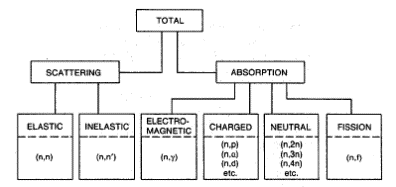
\includegraphics[scale=0.70]{image1.png}\\
\end{center}
\section{Mécanismes réactionnels}
La pluspart des réactions chimiques se produisent en une suite d'étape : \textbf{mécanisme réactionnel}.\\

\textbf{Attention !} Une réaction équilibrée donne les facteurs stœchiométriques et les réactifs / produits mais \textit{pas} le mécanisme!
\\
Définissions d'abord la \textbf{molécularité :} \textit{nombre de molécules qui doivent entrer en collision pour produire la réaction}.\\
Ainsi, une réaction élémentaire est une réaction dont l'équation de vitesse peut être exprimée à partir de sa molécularité.
\begin{center}
	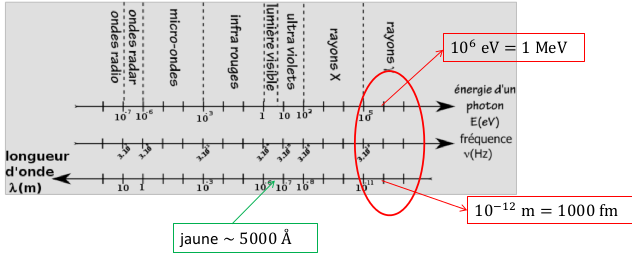
\includegraphics[scale=0.70]{image2.png}\\
\end{center}

Un mécanisme réactionnel doit satisfaire deux exigences :
\begin{enumerate}
	\item Somme des réactions élémentaires = équation équilibrée globale
	\item Mécanisme proposé conforme à l'équation de vitesse expérimentale
\end{enumerate}\ \\
Pour élaborer un mécanisme réactionnel il faut :
\begin{itemize}
	\item Déterminer expérimentalement la vitesse de la réaction globale
	\item Elaborer les mécanismes possibles
	\item Par l'expérience, écarter les mécanismes les moins probables
\end{itemize}


\section{Théorie des collisions}
On cherche à répondre à : \textit{"Comment se produit une réaction chimique ?"}\\
Expérimentalement, $k$ augmente avec la température. Pour l'expliquer, il existe une théorie nommée : \textit{théorie des collisions}.\\

Celle-ci stipule que l'augmentation de la vitesse des molécules du à l'accroissement de température augmente la fréquence de collision.\\

Bien que l'idée est sympa, on remarque que $r <<$ fréquences des collisions. C'est \textit{Arrhenius} qui, déclara que toutes les collisions ne sont et efficaces et qu'\textit{il existe un seuil à dépasser pour qu'il y ait réaction} $\Rightarrow$ \textbf{seuil d'activation} (ou \textbf{complexe activé}).\\

On remarque qu'à une T donnée, seule une certaine proportion des collisions possède une énergie $\geq E_a$. On peut déterminer ces collisions "utiles" : $n_{tot}\ collisions\ . exp(\frac{-E_a}{RT})$.\\

Comme si ce n'était pas suffisant, il faut également tenir compte de l'orientation des collisions : certains "chocs" étant propice à la réaction :
$$k = z\ p\ exp\ (\frac{-E_a}{RT})$$
\begin{itemize}
	\item[z] : fréquence des collisions
	\item[p] : facteur stérique = propension de collisions ayant une orientation favorable
\end{itemize}
D'ou on tire l'\textit{équation d'Arrhénius} :
$$k = A\ exp\ (\frac{-E_a}{RT})$$
où $A$ est le facteur de fréquence (déterminant les orientations favorables).

\subsection{Théorie du complexe activé ( = de l'état de transition)}
Théorie plus générale que la théorie des collisions, applicable en solution et en phase gazeuse. Elle décrit la rencontre entre les réactifs (= complexe activé) comme une structure lâche prête à former de produits. (lâche = qui passe de l'un à l'autre (réactif / produit).

\section{Catalyse}
Élever la température est un moyen pour accélérer une réaction mais ce n'est pas toujours faisable : on utilise dès lors des catalyseurs.\\
Un \textbf{catalyseur} est une substance permettant d'accélérer une réaction (sans être consommée par la réaction).\\
Ils fonctionnent en augmentant la proportions de collisions efficaces à une T donnée ou en donnant une nouvelle voie pour la réaction avec une $E_a$ plus faible.\\
Il en existe des \textit{homogènes} (dans la même phase que les molécules de réactifs et \textit{hétérogène} (dans une autre phase).


\newpage
\chapter{Électrochimie}
L'électrochimie est l'étude de la transformation de l'énergie chimique en énergie électrique et vice versa.

\section{Piles électrochimiques}
On va utiliser des réactions d'oxydoréduction (\textit{cf. confond}) pour produire du courant. Comment ? \\

En reliant deux compartiments contenant, par exemple, du $MnO_4^-$ et du $Fe^{2+}$. Le passage des $e^-$ par le fil permet de récupérer un travail utile \textbf{mais} il y a un problème d'accumulation de charge : mise en place d'un pont électrolytique (ou d'un disque poreux reliant les deux compartiments).\\
Cela permet de garder les solutions en contact, sans permettre le mélange complet et surtout, le déplacement possible des ions afin de respecter le bilan de charges.\\

Ainsi, une \textbf{pile électrochimique} est un dispositif dans lequel l'énergie chimique est transformée en énergie électrique. (Dont le processus inverse se nomme \textit{électrolise}). Notons que :
\begin{itemize}
	\item La réaction à lieu à la surface de l'électrode
	\item L'anode est l'électrode où à lieu l'oxydation
	\item La cathode est l'électrode où à lieu la réduction
\end{itemize}
\textbf{La force électromotrice (E)} (=DDP) est la force qui déplace les $e^-$ dans le fil conducteur d'un agent réducteur vers un agent oxydant. 

\section{Potentiel standard de l'électrode}
La force électromotrice est calculée en faisant la somme des potentiels des demi-réactions. Parfois, on peut mesurer le potentiel total mais pas celui des processus à chaque électrode.\\
Par convention  : On assigne un potentiel de $0 V$ à l'\textit{électrode normale d'hydrogène}.
$$2H^+ + 2e^- \rightarrow H_2\ \ \ \ [H^+] = 1M, p_{H_2} = 1\ atm$$
Supposons la pile avec la réaction $2H^+ + Zn \rightarrow Zn^{2+} + H_2$. Le potentiel total valant $0,76V$, en couplant cette demi-réaction avec celle de référence on peut assigner un potentiel à la demi-réaction (Valable $\forall$ demi-réaction)
$$E^0_{pile} = E^0_{H^+ \rightarrow H_2} + E^0_{Zn \rightarrow Zn^{2+}} = 0V + 0,76V = 0,76V$$
Connaissant le potentiel de la demi-réaction, on peut en calculer d'autre ! Par exemple, la pire $Zn + Cu^{2+} \rightarrow Zn^{2+} + Cu$
$$E^0_{pile} = 1,1V = E^0_{Zn \rightarrow Zn^{2+}}  E^0_{Cu^{2+} \rightarrow Cu}$$
Comme on a déterminé plus haut la valeur $0,76V$, on peut déduire que $E^0_{Cu^{2+} \rightarrow Cu} = 0,34V$. On peut ainsi retrouver tous les potentiels ! Youhou !\\

\textit{NB :} Le potentiel d'une demi réaction est toujours écrite sous la forme d'une réaction de \underline{réduction} ! Les potentiels standards, eux, sont défini à 1M et 1 atm. \\

De plus, inverser une des demi-réaction inverse le signe du potentiel. Cerise sur le gâteau, multiplier les demi-réactions par un facteur (équilibrage $e^-$) ne modifie \textbf{pas} le potentiel.

\subsection{Représentation schématique d'une pile}
Par exemple, prenons la pile :
$$Mg | Mg^{2+} || Al^{3+} | Al$$
Cette écriture dénonce la présence du compartiment anodique à gauche, du cathodique à droite. La double ligne verticale correspond à la séparation des compartiments (par un pont salin) et une ligne correspond à un changement de phase.

\subsection{Description complète d'une pile électrochimique}
Avant tout : \textit{le fonctionnement spontané d'une pile se fera si son potentiel est \textbf{positif}}.\\
Les facteurs à déterminé sont : sens de des $e^-$, anode, cathode, le potentiel et la réaction équilibrée de la pile. (Exemple de description \textit{slide 15})

\section{Potentiel d'une pile, travail électrique et énergie libre}
Il existe une relation thermo/électro. Le travail accompli par le déplacement des électrons dépend de la force agissant sur ceux-ci, qui est fonction de la différence de potentiel.\\
Le potentiel étant un travail sur une charge, on peut dire ($E = -\frac{W}{q}$)
\begin{itemize}
	\item Une pile électrochimique produit du courant à un potentiel E > 0
	\item Une pile électrochimique fournit un travail à un W < 0
\end{itemize}
\textit{NB :} Si transfert de $n$ moles d'$e^-$ : $q = nF$.\\

Petite parenthèse, voici la \textit{Loi de Faraday :}
$$N = \frac{RT}{nF}\ \ \ \ (N = n_{br}\ de\ moles\ \ \ n = n^{br}\ de\ moles\ d'e^-)$$
On se rend compte qu'on peut définir un travail maximum : $W_{max} = -qE_{max}$. Pour tirer un travail maximum, il faut un \textbf{processus réversible}. L'efficacité d'une pile sera ainsi définie comme $>/>_{max}$.
\subsection*{Relation potentiel et Gibbs}
$$W_{max} = \Delta G \rightarrow \Delta G = -qE_{max} = -nFE_{max}$$
Cette relation est valable aussi pour $\Delta G^0$ et fournit un moyen expérimental de mesure de $\Delta G$. De plus, elle démontre le fonctionnement spontanné d'une pile ($\Delta G <0 \Leftrightarrow E > 0$).

\section{Influence de la concentration sur le potentiel d'une pile}
Une pile de concentration est une pile dont les deux compartiments contiennent les mêmes sels mais à des concentrations différentes. 
\begin{wrapfigure}[6]{l}{3cm}
	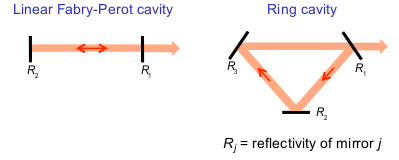
\includegraphics[width=3cm]{image3.png}
\end{wrapfigure}

Les électrons vont se déplacer de sorte à atteindre l'équilibre des concentrations. Dans le cas ci-contre, les $e^-$ vont aller de gauche à droite pour :
\begin{itemize}
	\item Oxydation à gauche ($Ag \rightarrow Ag^+ + e^-$) $\Rightarrow$ Augmentation $Ag^+$.
	\item Réduction à droite ($Ag^+ +e^- \rightarrow Ag$) $\Rightarrow$ Diminution $Ag^+$.
\end{itemize}
\subsection*{Équation de Nernst}
Sachant que $\Delta G = \Delta G^0 + RTln(Q)$ et $\Delta G = -nFE$ on peut écrire : 
$$\Delta G^0 + RTln(Q) = -nFE \Rightarrow E = E^0 - \frac{RT}{nF}ln(Q)$$
Ce qui donne à 25 degrés (Attention, c'est un log !)
$$E = E^0 - \frac{0,0592}{n}log(Q)$$
Cette équation permet le calcul du potentiel d'une pile pour des étants non standard.\\

Le $E$ calculé par Nernst est le potentiel maximal avant toute production de courant. La décharge de la pile (courant anode vers cathode) fait varier les concentration et donc E jusqu'à attendre l'équilibre : Q = K, d'où $\Delta G = 0$ et la \textbf{pile est à plat}.
$$E = 0 = E^0 - \frac{RT}{nF}ln(K)$$
On peut dès lors mesurer le pH via des électrode de référence (Voir \textbf{labo 1, slide 24 - 25}).

\section{Accumulateur}
Un accumulateur est un appareil emmagasinant de l'énergie électrique sous forme chimique.
\subsection*{Batterie au plomb}
Pour recharger la batterie, il faut appliquer une réaction inverse. Recharger une batterie déchargée par cable est dangereuse : La circulation du courant peut amener à l'électrolyse de l'eau, former un arc électrique pouvant exploser la batterie ! Il faut donc connecter une prise terre.\\
Théoriquement, on peut recharger un nombre illimité de fois la batterie mais à cause des chocs ce n'est pas le cas.

\subsection*{Piles sèches et à combustible}
\textit{Cf. slide 29 - 32}

\section{Corrosion}
Il s'agit d'un processus spontané inverse de la séparation d'un métal en son minerai. \textbf{La corrosion est l'oxydation d'un métal}.

\subsection*{Prévention de la corrosion}
La plupart des métaux sont recouvert d'une couche d'oxyde au potentiel supérieur à $O_2$ empêchant l'oxydation des atomes internes. Certaines peintures peuvent aussi freiner la corrosion.\\

\begin{wrapfigure}[6]{l}{3cm}
	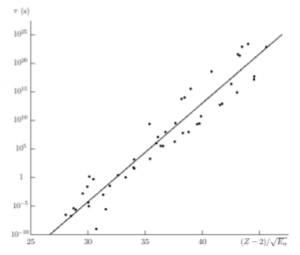
\includegraphics[width=3cm]{image4.png}
\end{wrapfigure}
Une autre méthode est la \textit{galvanisation de l'acier} : ce-dernier va  se "sacrifier" grâce à un potentiel plus bas que le métaux que l'on veut protéger : il joue le rôle d'\textit{anode sacrificielle}. Dans le schéma ci-contre, l'anode (magnésium) joue ce rôle. Attention : quand l'anode est totalement sacrifiée, il faut la remplacer sinon c'est la tuyauterie qui se fera manger.

\section{Électrolyse}
Il s'agit du processus inverse à la pile : il faut dans ce cas utiliser de l'énergie électrique pour provoquer une réaction chimique $\Rightarrow E^0 <0$. C'est un processus \textbf{non-spontané}.

\subsection*{Caractéristiques stœchiométriques des processus électrolytiques}
Avant tout, une petite définition : \textit{Le plaquage est un procédé au cours duquel un métal se dépose sur une électrode par \underline{réduction} des ions métalliques présents dans la solution}. Voici un exemple ou il est d'application :\\

"\textit{Calcul de la masse de $Zn$ déposée dans une cellule électrolytique après passage d'un courant de $10,0A$ pendant $30,0\ min$."}
\begin{enumerate}
	\item Recherche de la réaction à la \underline{cathode} [$Zn^{2+} + 2e^- \rightarrow Zn$]
	\item Calcul de la charge transférée [$q = I.t$]
	\item Calcul du nombre de moles d'$e^-$ transférées [$n(e^-) = n.\frac{1}{F} $]
	\item Calcul du nombre de moles de $Zn$ déposé. [$n(Zn) = n(e^-).\frac{1\ mol\ Zn}{2\ mol\ e^-}$]
	\item Calcul de la masse de $Zn$ déposé. [$m(Zn) = n(Zn).M(Zn)$]
\end{enumerate}

\subsection{Électrolyse de l'eau}
C'est le processus inverse de la pile à combustible utilisant la réaction spontannée : 
$$2H_2 (g) + O_2 (g) \rightarrow 2 H_2O (l)$$
Elle se caractérise par les demis réactions :
\begin{itemize}
	\item \textbf{Anode :} $2H_2O \rightarrow O_2 + 4H^+ + 4e^-$
	\item \textbf{Cathode :} $4 H_2O + 4e^- \rightarrow 2 H_2 + 4 OH^-$
\end{itemize}
Des électrodes de platine dans l'eau pure ne font rien (trop peu d'ions). Mais dès qu'un peu de sol soluble est ajouté, il y a apparition de bulles d'$O_2$ et de $H_2$.\\

La réaction globale de l'eau est : 
$$6 H_2O \rightarrow 2 H_2 + O_2 + 4(H^+ + OH^-) \Rightarrow 2 H_2O \rightarrow 2 H_2 + O_2$$
et son potentiel vaut : $E = -1,23 V$.

\subsection{Électrolyse d'un mélange d'ions}
\textit{Cf. slide 45}\\
La fin du chapitre (\textit{slide 46 - 55}) n'est pas à étudier.

\newpage
\chapter{Structure de l'atome}
\section*{Introduction}
Le concept d'atome vient de la supposition de l'existence d'une particule indivisible. Bien plus tard, Dalton proposa une théorie atomique :
\begin{enumerate}
	\item Chaque élément est formé d'atomes
	\item Les atomes d'un élément donné sont identiques
	\item Formation de composé chimique quand combinaison des atomes
	\item Réorganisation des atomes lors d'une réaction chimique
\end{enumerate}
\ \\
Début du 20$^e$ siècle, Thomson détermine expérimentalement le rapport charge/masse d'un électron. En 1909, Millikan découvrit la charge de l'électron et d'en déduire sa masse.\\
Vient ensuite Rutherford avec son plum-pudding jusqu'à arriver à la théorie moderne de la structure atomique : On lie les ondes et les particules, il y a dualité onde-corpuscule : explication de la périodicité des propriétés chimiques des éléments par la configuration électronique.

\section{Radiation électromagnétique}
Une radiation électromagnétique est une des forme de déplacement de l'énergie. Pour la caractériser, on défini la longueur d'onde $\lambda$ qui est la distance entre deux crêtes, la fréquence, la vitesse (= $c$) et la relation : $\lambda v = c$.

\section{Nature de la matière}
Max Plank découvre en prenant des solides à incandescence que la lumière qu'ils émettent, l'énergie transférée n'est pas dans un continuum. Il remarque qu'il y a quantification de l'énergie : celle-ci est transférée sous forme de multiples entier (un quantum).
$$1\ quantum\ =\ hv$$
On peut de la définir la variation d'énergie d'un système : $\Delta E : n h v$ où $n \in \mathbb{N}$. L'énergie est donc transférée en quanta entiers et celle-ci est dotée de propriétés corpusculaires.\\

Albert Einstein proposé ensuite que les radiations électromagnétiques sont un flux de particules ; de photons.
$$E_{photon} = h v = h\frac{c}{\lambda}$$
Celui-ci nous appris également que l'énergie possède une certaine masse via la théorie de la relativité restreinte $\Rightarrow E = mc^2$.\\

C'est plus tard que de Broglie associa les particules à des ondes (\textit{Cf. Physique générale}.\\
En calculant la longueur d'onde d'un électron, on a pu se rendre compte qu'il existe une certaine distance entre les atomes dans un cristal. Ceci a été mis en évidence par la diffraction : \textit{dispersion de la lumière par un agencement régulier de points ou de lignes}.\\

Le fait que la lumière se diffracte (sillon d'un CD) met en évidence le caractère ondulatoire de la lumière (seule les ondes pouvant se diffracté). Toutes les particules de matières possèdent donc à la fois des caractéristiques ondulatoires et corpusculaires.

\section{Spectre de l'atome d'hydrogène}
En exposant $H_2$ gazeux à une forte décharge électrique, on excite les atomes qui libèrent de la lumière donnant lieu au spectre d'émission de l'atome hydrogène.
On peut également obtenir un spectre en faisant passer de la lumière blanche à travers un prise. Celui-ci sera constitué de \textbf{toutes} les longueurs d'onde de la lumière visible.\\

Par contre, les spectres de raies ne permet la visualisation que pour certaines longueurs d'ondes, ce qui est $\neq$ du spectre continu.Par exemple, le spectre d'émission de $H$ est un spectre de raie car on a accès à certains niveaux d'énergie seulement.

\section{Modèle atomique de Bohr}
Bohr émet l'hypothèse que l'$e^-$ de $H$ ne gravite que selon certaines orbites circulaires bien déterminées, et qu'il est impossible de construire un modèle de $H$ en se basant sur la physique classique.\\
En prenant en compte les résultats expérimentaux de l'atome de $H$, il défini les niveaux d'énergie accessible par $e^-$ :
$$E = -2,718*10^{-18} \frac{Z^2}{n^2}\ [J]$$
où $n \in \mathbb{N}$ et $Z$ est la charge du noyau (si $n = \infty, E = 0$).\\
Cette relation permet de calcul de la variation d'énergie, de la longueur d'onde de la lumière absorbée (ou émise) lorsqu'un électron change d'orbite (Perte d'énergie = signe négatif = état plus stable (libération photon)).\\

Ce modèle fonctionne bien pour l'atome $H$ mais pas du tout pour les autres (gros bad).

\section{Modèle atomique basé sur la mécanique ondulatoire}
Se rendant compte qu'ils étaient dans une belle merde, Heisenberg, de Broglie et Schrödinger sont arrivés en héros en mettant en place la mécanique quantique.\\

De Broglie mis en évidence des propriété ondulatoire de $e^-$ et à ensuite formulé avec Schödinger l'hypothèse que l'électron est lié au noyau est assimilable à une onde stationnaire. D'ailleurs, voici son équation  :
$$H\psi = E\psi$$
Le $\psi$ représente la fonction d'onde (coordonnées dans l'espace). Cette fonction mise au carée indique la probabilité de trouver un électron en ce point de l'espace. $H$ est un opérateur mathématique et $E$ est l'énergie totale de l'atome.\\
Une solution de cette équation donne une fonction d'onde associée à une valeur de $E$.\\

\textbf{Attention ! } Il ne faut pas confondre \textit{orbitale} (désigne une zone de probabilité de présence) et \textit{orbite} (de Bohr). Niveau déplacement des $e^)$, on ne sait pas.\\

Comme on a remarqué qu'on ne savait pas grand chose, Heisenberg à mis en place un principe d'incertitude :
$$\Delta x . \Delta (mv) \geq \frac{h}{4\pi}$$
où $\Delta x$ est l'incertitude relative à la position, $\Delta (mv)$ est l'incertitude relative à sa quantité de mouvement et $h$ la constante de Planck.\\
Cela signifie que que \textit{plus on connaît avec précision la position d'une particule, moins on connaît avec précision sa vitesse, et vice versa.}. Pour conséquence, on ne peut connaître avec précision la trajectoire de l'électron autour du noyau.\\

Pour représenter $\psi^2$, on a le choix entre une distribution radiale en fonction de $r$ par exemple.

\section{Nombres quantiques}
Une orbitale = une série de nombre quantique.
\begin{enumerate}
	\item Nombre quantique principal $n$ ; Définit la taille de l'orbitale ($n = 1, 2, 3, ...$)
	\item Nombre quantique secondaire ou azimutal $l$ ; Définit la forme de l'orbitale ($l \in [0, n-1]$)
	\item Nombre quantique magnétique $m_l$ ; Définit l'orientation de l'orbitale par rapport à cell des autres orbitales ($m_l \in [-m, m]$)
\end{enumerate}
\textit{NB  :} une sous-couche est l'ensemble des orbitales correspondant à une même valeur de $l$.

\section{Formes des orbitales et niveaux d'énergie}
\begin{wrapfigure}[8]{l}{2,7cm}
	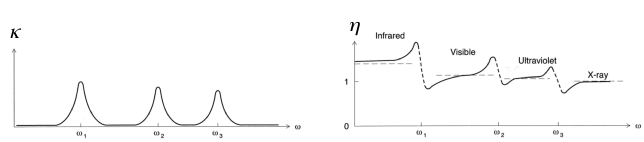
\includegraphics[width=2.5cm]{image5.png}
\end{wrapfigure}
Ci-contre la réprésentation des orbitales $1s, 2s$ et $3s$ de l'atome H. Le $a)$ représenta la probabité de trouver la présence d'électrons alors que $b)$ représente la surface externe englobant $90\%$ de la probabilité de présence d'un $e^-$.\\
Les zones nodales (nœuds) sont les zones de probabilité nulles ($n-1$ zone nodale dans les orbitales $s$).
Pour les orbitales $2p$, la forme est celle de deux lobes. Pour les autres, \textit{la forme n'est pas importante}.\\
L'énergie des orbitales est fonction de $n$ uniquement ; même $n$ = même énergie = \textit{dégénérescence}.

\section{Spin de l'électron et principe d'exclusion de Pauli}
S. Goudsmit propose que l'électron tourne sur lui même en vue du résultat donné par les spectres : ajout d'un $4^e$ nombre quantique : le nombre quantique de spin $m_s$.\\
Le principe d'exculsionde Pauli : 
\begin{center}
	\textit{Dans un atome donné, deux électrons ne peuvent pas être caractérisé par le même ensemble de nombre quantique ($n, l, m_l, m_s$)}
\end{center}
C'est à dire qu'un $e^-$ d'une même orbitale à les mêmes valeurs $n, l, m_l$ mais \textbf{pas} $m_s$. Une orbitale peut comporter au plus deux $e^-$ qui doivent être de spin opposés (fondamental pour construire le tableau périodique)

\section{Atomes polyélectroniques}
L'équation de Schrödinger fonctionnait bien pour H, mais impossible de la résoudre exactement pour les autres car pour ça il faudrait connaître l'énergie cinétique des électrons, l'énergie d'attraction potentielle entre $e^-$ et le noyau et l'énergie de répulsion potentielle entre les $e^-$. On va donc devoir approximer.\\

On va émettre l'hypothèse que chaque $e^-$ se déplace dans un champ électrique qui est la résultante de l'attraction par le noyau et de la répulsion moyenne. Ces orbitales hydrogénoïdes auront ainsi la même forme que les orbitales de H, mais différentes par leurs tailles et énergie (et elles tiennent compte de la fameuse hypothèse)\\

$\Rightarrow$ Dans H, toutes les orbitales de même $n$ ont des énergies semblables mais dans les atomes polyélectronique, les orbitales de mêmes $n$ on est énergies différentes.

\section{Historique du tableau périodique}
En essayant de mettre en évidence des similitudes entre les propriétés chimiques de certains éléments, Mendeleïev a été capable d'aller jusqu'à prédire l'existence et la propriétés d'éléments pas encore découvert ! 

\section{Principe du \textit{aufbau} et tableau périodique}
La configuration électroniques des orbitales hydrogénoïdes permet d'expliquer l'organisation du tableau périodique par le principe de \textit{aufbau} : construction par empilement.\\
Le pricipe est d'ajouter des $e^-$ un à un aux orbitales hydrogénoïdes. En gros il faut constuire les atomes en remplissant des petites cases et en tenant compte du Spin $\rightarrow$ voir en TP.\\
\begin{wrapfigure}[6]{l}{2,7cm}
	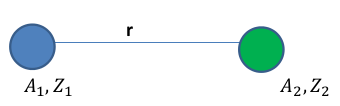
\includegraphics[width=2.5cm]{image6.png}
\end{wrapfigure}
Notons quand même la règle de Hund : 

\textit{Pour un atome, la configuration de moindre énergie est celle pour laquelle, dans un ensemble donné d'orbitales dégénérées, il y a le plus grand nombre possible d'électrons célibataires permis, conformément au principe d'exclusion de Pauli. Tous ces électrons célibataires ont des spins parallèles.}

Pour parfois alléger les notation, on se base sur la configuration d'un gaz rare : \textit{configuration de coeur}.

\subsection{Configuration électronique des éléments}
Les électrons de valence sont les électrons dont le nombre quantique principal est le plus élevé dans un atome donné : ce sont eux qui interviennent dans les réactions chimiques.\\
Les électrons de la couche internes : électrons de cœur. Pour le tableau, les éléments d'un même groupe ont la même configuration au niveau des $e^-$ de valence ainsi que des comportements chimiques semblables.

\section{Périodicité des propriétés atomiques}
L'énergie d'ionisation est l'énergie requise pour arracher un $e^-$ d'un atome ou d'un ion à l'état gazeux  (pour former un ion positif); celle-ci est plus forte pour les $e^-$de cœur.
$$A_g \rightarrow A_g^+ + e^-$$

L'affinité électronique est la quantité d'énergie associée à l'addition d'un électron à un atome à l'état gazeux. La configuration électronique influence cette affinité.\\
En général, dans un même groupe, quand $Z$ augmente, l'affinité électrique fait de même.\\

Par contre, cela n'explique pas la dimension précise des orbitales ni de l'atome. Comment ont-ils dès lors calculés ça ? \\
Le rayon atomique est la demi-distance séparant les atomes (identiques) d'une molécules. En général, quand $Z$ augmente : 
\begin{itemize}
	\item Dans une même période, le rayon atomique diminue (la charge du noyau augmentant, les $e^-$ de valence sont plus fortement attirés)
	\item Dans un même groupe, le rayon atomique augmente (La tailles des orbitales augmente)
\end{itemize}

\section{Propriétés des éléments d'un groupe donné : les métaux alcalins}
Le tableau périodique est conçu pour mettre en évidence toutes similitudes de propriétés entre les éléments. On y retrouve notamment une distinction métal - non métal : 

\begin{enumerate}
	\item Non métal : Tendance à céder des $e^-$ pour former des cations stables. Ils ont en général une faible énergie d'ionisation et les plus réactifs sont dans le coin inférieur gauche.
	\item Non métal : Tendance à accepter des $e^-$ pour former des cations stables. Ils ont en générale une énergie d'ionisation très élevée.
\end{enumerate}

\newpage

\chapter{Liaisons chimiques}
La façon dont les atomes sont liés les uns aux autres dont un composé chimique est l'objet de ce chapitre.

\section{Types de liaisons chimiques}
Une liaison chimique est une force qui retient un groupe d'atomes ensemble. Inversement, l'énergie de liaison est l'énergie nécessaire pour rompre une liaison.\\
\textbf{Attention !} Un type de liaison chimique est une attraction entre deux atomes, et pas une réaction pour former des ions de charges opposées.\\\\
\textit{NB :} Si deux atomes $H$ s'attirent pour former $H_2$, c'est parce qu'ensemble ils possèdent un état d'énergie moindre. Dans ce cas, la distance est telle que l'énergie minimale est la longueur de la liaison.\\

Une \textit{liaison ionique} se manifeste par réaction entre un atome cédant facilement des $e^-$ et un atome dont l'affinité pour les $e^-$ est élevée (typiquement métal - non métal).\\
Ceci entraine à la formation d'un composé ionique qui a atteint le niveau d'énergie le plus bas.\\
La \textit{liaison covalente} est le partage des électrons par les noyaux. Ces deux liaisons sont des états extrêmes et il existe d'autres cas comme la \textit{liaison covalente polaire}.

\section{Électronégativité}
Il s'agit de la capacité d'attraction d'un atome envers les électrons de liaisons. On la définit par une valeur $\in [0.7, 4.0]$.\\
Dans une même période, l'électronégativité augmente avec $Z$ alors que dans un même groupe elle diminue avec $Z$.

\section{Polarité de la liaison et moments dipolaires}
Certaines molécules ont une distribution de charges telle qu'elles possèdent un moment dipolaire (Une liaison polaire dans une molécule diatomique en a toujours un).\\
Les liaison polaires \textit{peuvent} produire un moment dipolaire : $H_2O$ (mais pas $CO_2$).\\
Le moment dipolaire peut s'annuler si les polarités des différentes liaisons font de même.

\section{Configurations électroniques et tailles de ions}
Un atome d'un composé stable à presque toujours la configuration électronique d'un gaz rare ; la réaction entre deux non-métaux (covalente) ou non-métal / métal (covalente).\\

Le terme \textit{composé ionique} se réfère à l'état solide (état ou les ions sont regroupés afin de minimiser les répulsions (très différent de gazeux)) de ce composé.\\

La taille joue également un rôle important au niveau structure, stabilité et propriété. Comme pour les atomes, leur taille est déterminée à partir de la distance mesurée entre centres des ions d'un composé ionique.

\begin{enumerate}
	\item \textbf{Cation} ; perte de $e^- \Rightarrow$ Plus petit que l'atome
	\item \textbf{Anion} : gain de $e^- \Rightarrow$ Plus grand que l'atome
\end{enumerate}

\section{Composés ioniques binaires}
Si possibilité d'être plus stable $\rightarrow$ formation d'un solide ionique.\\
L'\textit{énergie de réseau} est la variation d'énergie accompagnant la transformations d'ions individuels à l'état gazeux en un état solide ionique : 
$$A^+_g + X^-_g \rightarrow AX_s$$
Celle-ci caractérise la force d'attraction que les ions exercent les uns sur les autres : valeur négative : processus endothermique (\textit{Cf. exemple slide 17}).\\
L'énergie de réseau se définit : 
$$E = k \frac{Q_1 Q_2}{r}$$
ou $k$ est une constante dépendant de la structure du solide et de la configuration électroniques alors que $Q_1$ et $Q_2$ sont les charges des ions et $r$ la distances anions / cations.\\
Comme mentionné ci-dessus, ce sera exothermique si les charges sont opposées.

\section{Caractère partiellement ionique des liaison covalentes}
Atome d'électronégativité = partage égal des électrons dans une liaison covalente. Mais tout ne se fait pas toujours à l'amiable et il y a des atomes d'électronégativité différente = partage inégal des électrons de liaisons. Deux cas possible : 
\begin{enumerate}
	\item Formation d'une liaison covalente polaire.
	\item Formation d'une liaison ionique si différence d'électronégativité très grande.
\end{enumerate}
Une difficulté pour définir des composés ioniques et la présence des ions polyatomiques ($NH_4^+$ par exemple). La définition officielle devient donc : 
\begin{center}
	\textit{Tout solide qui, fondu ou dissous dans l'eau, permet le passage du courant électrique est un composé ionique}.
\end{center}

\section{Liaisons covalentes : un modèle théorique}
Encore une fois, il n'y aura formation d'une liaison chimique que si les atomes sont plus stables groupés que séparés. Par exemple : 
$$CH_4 \rightarrow C + 4H\ \ \ \ \ \ \ \Delta H = + 1652\ kJ$$
Il faut donc fournir de l'énergie pour briser les liaisons.
$$CH_4 + 4H \rightarrow C + CH_4\ \ \ \ \ \ \ \Delta H = - 1652\ kJ$$
Ici, on libère de l'énergie pour la formation de la molécule stable $CH_4$.\\

Le concept de liaison est une représentation de la distribution de l'énergie associée à la formation d'une molécule stable à partir de ses atomes constituants.\\
S'il y a partage des $e^-$ on peut supposer qu'il existe des \textit{liaison individuelles entres paries d'atomes} (On étudie par paire de liaisons plutôt que atome par atome car plus simple).\\

Les valeurs expérimentales confirment l'existence de ces "liaisons discrètes" indépendants de leur environnement moléculaire.

\section{Énergies des liaisons covalentes et réactions chimiques}
On se rend compte que ces liaisons ne sont pas si indépendantes que ça au niveau de l'environnement moléculaire : on considèrera dès lors une énergie de liaison moyenne.\\
Il existe bien sur plusieurs types de liaisons : 
\begin{enumerate}
	\item \textbf{Liaisons simples} : liaison comportant une seule paire d$e^-$ de liaison
	\item \textbf{Liaisons multiples} : doubles (2 paires d'$e^-$), triples (3 paires d'$e^-$)
\end{enumerate}
L'augmentation du nombres de paires d'$e^-$ augmente l'énergie de liaison mais diminue la longueur de la liaison.\\
\textit{NB : } On peut utiliser les énergies de liaison pour calculer approximativement la variation d'enthalpie d'une réaction.

\section{Théories des électrons localisés}
Théorie décrivant la liaison covalente en stipulant qu'une molécule est composée d'atome retenus ensemble par le partage de doublet d'électrons. 
\begin{enumerate}
	\item \textbf{doublet libre} : paire d'$e^-$ appartenant à un seul atome
	\item \textbf{doublets liants} : paire d'$e^-$ partagés par deux atomes.
\end{enumerate}

\section{Diagrammes de Lewis}
Il s'agit de le répartition des $e^-$ de valence (et que eux) entre les atomes d'une molécule. Le principe est qu'un composé stable à une configuration semblable à un gaz rare (qui eu ont une couche de valence déjà remplie et ne forme pas de liaison).\\

Pour les non-métaux de la 2$^e$ période, il faut satisfaire la règle de l'octet à savoir posséder 8 $e^-$ sur sa couche de valence.\\
Règles des diagrammes de Lewis :
\begin{enumerate}
	\item Faire la somme des $e^-$ de valence de \textsc{tous} les atomes
	\item Utiliser un doublet d'$e^-$ pour former une liaison entre chaque paire d'atomes liés
	\item Répartir les $e^-$ résiduels avec le respect de la règle du doublet (H) et de la règle de l'octet (élem. 2$^e$ période).
\end{enumerate}
Voici des exemples copié-collé en HD : 
\begin{center}
	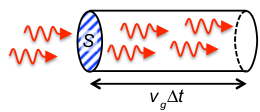
\includegraphics[scale=0.85]{image7.png}\\
\end{center}

\section{Exceptions à la règle de l'octet}
\subsection{Cas 1 :  Tendance à former un octet incomplet (< 8 électrons)}
\begin{wrapfigure}[4]{l}{1,5cm}
	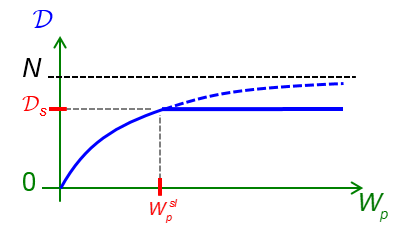
\includegraphics[width=1.5cm]{image8.png}
\end{wrapfigure}
Par exemple, le $BF_3$. Étant très réactif, il réagit violemment avec des molécules possédant des doublets libres.\\
L'atome de bore va devenir déficient en électrons : $\sum e^-_{val} = 24 e^-$.\\
On voit sur le diagramme ci-contre que $B$ ne possède que six électrons.

\subsection{Cas 2 :  Tendance à former un octet 'surcomplet' (> 8 électrons)}
\begin{wrapfigure}[6]{l}{1,5cm}
	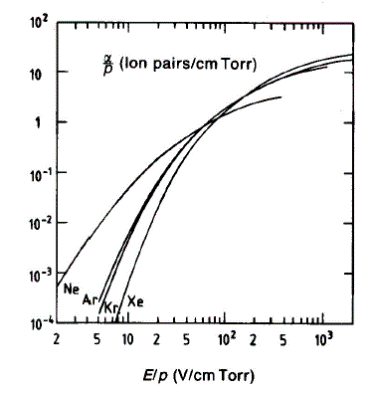
\includegraphics[width=1.5cm]{image9.png}
\end{wrapfigure}
Cas des éléments de la troisième période (et plus) qui on comme orbitale de valence en $3s, 3p$ et $3d$. Par exemple le $SF_6$, une molécule très stable\\
$\Rightarrow \sum e^-_{val} = 48 e^-$.\\
On voit sur le diagramme ci-contre que $S$ possède que 12 électrons !\\

\textit{NB :} On applique la règle de l'octet à ch acun des atomes et en cas d'$e^-$ résiduels on les place sur les orbitales $d$ non-occupée. Si $> 8 e^-$ à attribuer, on les assignes à l'atome central.
\newpage
\section{Résonance}
Parfois, plusieurs diagrammes de Lewis sont possibles. Par exemple, our l'ion nitrate $NO_3^-$, il  n'y a pas de raison d'assigner la liaison double à un $O$ en particulier :
\begin{center}
	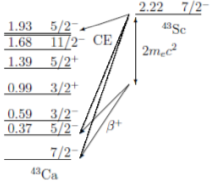
\includegraphics[scale=0.55]{image10.png}\\
\end{center}
La structure électronique sera donnée par la moyenne des structures de résonance.\\
Certaines molécules à nombre impair possède aussi des structures de résonance.\\

\subsection{Charge formelle}
Comment choisir quel diagramme retenir ? Pour faire ce choix, on va utiliser le concept de charge formelle.
La \textit{charge formelle} est la différence entre le nombre d'$e^-$ de valence sur l'atome neutre et le nombre d'$e^-$ de valence assignés à cet atome dans la molécule.\\
On suivra le mode d'emploi :
\begin{itemize}
	\item doublets libres : appartiennent aux atomes qui les portent
	\item doublets liants : répartis équitablement entre les deux atomes de la liaison
	\item $\Rightarrow$ le nombre d'$e^-$ assignés = $e^-$ doublet libre + $1/2\ e^-$ partagés.
\end{itemize}
La somme des charges formelle de tous les atomes dans une molécule ou un ion donne la charge globale de cette espèce.\\
En guise d'exemple, j'inclus ici le slide 43.\\
\begin{center}
	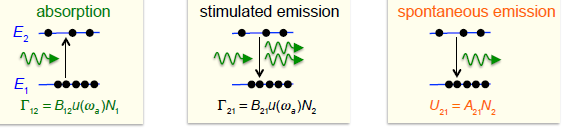
\includegraphics[scale=0.55]{image11.png}\\
\end{center}
Le choix du diagramme de Lewis le plus approprié sera celui pour lequel les atomes prennent les charges formelles le plus proche de 0, avec les charges formelles négatives appartenant aux atomes les plus électronégatif.

\newpage
\section{Structure moléculaire : théorie RPEV}
La structure moléculaire est un agencement tridimensionnel des atomes qui permet d'expliquer bon nombre de propriétés chimiques. La plus simple de ces théories est la \textit{théorie de répulsions des paires d'électrons de valence} ou RPEV pour les purs.\\

Un postulat est à tenir en compte :
\begin{center}
	\textit{L'agencement des électrons d'un atome donné est celui pour lequel la répulsion entre les doublets d'électrons est minimale.}\end{center}
	Marche à suivre : 
	\begin{enumerate}
		\item Écrire le diagramme de Lewis de la molécule
		\item Calculer le nombre de doublets d'électrons et les disposer afin de minimuser leur répulsion
		\item Déterminer la position des atomes en fonction de celle des doublets d'$e^-$
		\item Nommer la structure moléculaire découlant de la position des atomes et \textsc{pas} des doublets
	\end{enumerate}
	\textit{Pour les exemples, cf. slides 46 - 49}\\
	
	Les angles de liaisons sont présent pour éloigner au maximum les doublets : forcément, plus il y a de doublets plus l'angle de liaison diminue. Les différentes structures sont reprise ci-dessous : 
	\begin{center}
		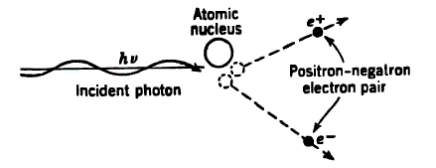
\includegraphics[scale=0.55]{image12.png}\\
	\end{center}
	Pour le cas des liaisons multiples, la règle générale est que cela correspond à un doublet d'$e^-$ effectif.
	
	
	\section{Hybridation et théorie des électrons localisés}
	Pour après Pâques ! 
	
	\chapter{Solides, liquides et gaz}
	\section{Forces intermoléculaires}
	La formation de molécules se fait grâce aux liaison intramoléculaires. Dans un solide, elle sera due à des liaisons ioniques ou covalentes et, dans certains cas, aux forces intermoléculaires (beaucoup plus faible).\\
	
	Dans un changement d'état, il y a bien modification des forces intermoléculaires mais \textbf{pas} des liaisons \textbf{intra}moléculaires (l'eau reste toujours de l'eau).\\
	On peut compter deux grands types de forces intermoléculaires
	\subsection*{Forces de London}
	Dans les gaz rares, les électrons sont répartis uniformément autour du noyau mais parfois la répartition n'est pas symétrique et crée un moment dipolaire temporaire. Ce dipôle induit son voisin et crée une force inter atomiques de faible intensité et de courte durée : \textit{la force dispersive de London}.\\
	
	Cette force existe également dans les molécules (plus elle possède d'$e^-$, plus la molécule est polarisable (justifie l'augmentation des points d'ébullition des hydrures).\\
	Notons que si le numéro atomique augmente, le nombre d'électrons fait de même et la chance d'avoir un dipôle sont plus élevées : forces de London.
	
	\subsection*{Forces dipôles - dipôles}
	Beaucoup de molécules possèdent un moment dipolaire. Les molécules polaires subissent ainsi des attractions électrostatiques entres elles (ces forces diminue si la distance entre les dipôles augmente).\\
	
	La liaison hydrogène avec $N, O, F$ suivent ce type de liaison. Ce sont les interactions dipôles-dipôles les plus forte : polarité élevée de la liaison et grand rapprochement des dipôles du à la petite taille de $N, O$ et $F$.
	
	\section{État liquide}
	La \textbf{tension superficielle} est la résistance qu'oppose un liquide à l'augmentation de sa surface, qui est d'autant plus élevée si les forces intermoléculaires sont importantes.\\
	
	La \textbf{capillarité} est l'ascension spontanée d'un liquide dans un tube capillaire.
	\begin{description}
		\item[Forces de cohésion] forces intermoléculaires tendant à diminuer la surface du liquide
		\item[Forces d'adhésion] interaction des molécules du solide avec celles de la paroi (par exemple le verre et l'eau). (contrée par les forces de cohésion)
	\end{description}
	\ \\
	Si le tube est capillaire (petit $\phi$) les forces d'adhésion > forces de cohésion et le liquide monte dans le tube.
	
	\subsection*{Capillarité}
	Le ménisque aura une forme \textit{concave} si adhésion > cohésion (eau) et une forme \textit{convexe} dans le cas inverse (mercure).
	
	\subsection*{Viscosité}
	Il s'agit de la mesure de la résistance d'un liquide à l'écoulement (liaison $O-H$ augmente la viscosité).
	
	\section{Introduction à l'étude des structures et des types de solides}
	Il y a deux grandes catégories de solides : 
	\begin{description}
		\item[cristallins] Possèdent un assemblage régulier. Représentation à l'aide d'un réseau. Une maille est la plus petite unité de réseau.
		\item[amorphes] Désordre de leur structure, composants \textit{figé sur place} sans s'assembler comme des légos.
	\end{description}
	
	\subsection*{Analyse des solides par diffraction des rayons X}
	En envoyant des rayons X, on peut observer la diffraction : production d'interférences constructives et destructives.\\
	Les interférences seront constructives $\Leftrightarrow$ la distance additionnelle parcourue par l'onde inférieure est un multiple de la longueur d'onde.
	$$xy + yz = n\lambda$$
	Comme $nx + yz = 2D\sin \theta$, on peut trouver la \textbf{relation de Bragg} (où $d$ est la distance inter-atomiques calculable informatiquement) :
	$$n\lambda = 2d\sin \theta$$
	Le diffractomètre impose des rotations permettant l'enregistrement de pics de diffractions différentes permettant l'analyse du solide.
	
	\subsection*{Types de solides cristallins}
	Pour notre plus grand bonheur, il en existe plusieurs.
	\begin{description}
		\item[Solides ioniques] Les nœuds du réseau sont les ions qui, dissous dans l'eau est électrolyte 
		\item[Solides moléculaires] Les nœuds de réseau sont les molécules covalente qui, dissoute dans l'eau, ne sont pas électrolytes.
		\item[Solides atomiques] Les nœuds de réseau sont des atomes (tous les métaux). Ils sont classés en plusieurs srotes
		\begin{enumerate}
			\item solides métalliques : possède des liaison métalliques (= covalente délocalisée)
			\item solides covalents : fortes liaison covalentes délocalisée et orientée
		\end{enumerate}
	\end{description}
	\textsc{Inclure tableau comparatif slide 16.}
	
	
	\section{Structure et liaison dans les métaux}
	On peut retrouver deux sortes d'empilement donnant lieux ou a un réseau hexagonal compat (hc) ou à un réseau cubique à face centrée (cfc). Dans les deux cas, chaque sphère est entourée de 12 sphères.\\
	\textit{Voir slide 20 sur les mailles élémentaires, c'est plus du détail mais c'est toujours intéressant !}
	
	\subsection*{Théorie de la mer d'électrons}
	Rappelons d'abord que la liaison entre atomes dans la métaux est forte et \textbf{non} orientée.\\
	
	L'idée est que le réseau de cation métallique baigne dans une mer d'électron de valence. Quand les $e^-$ bougent, ils conduisent de la chaleur et de l'électricité (les cations se déplacent facilement lorsque l'on tréfile le métal).
	
	\subsection*{Théorie des bandes d'énergie}
	Basée sur les orbitales moléculaires, elle stipule que les électrons se déplacement dans l'ensemble du cristal métallique dans des OM formée à partir des orbitales des $e^-$ de valence des atomes métalliques.\\
	La différence entre l'OM liante et l'OM antiliante met en avant des \textit{bandes d'énergie} quand les OM sont très nombreuses et voisines.
	
	\subsection*{Alliages métalliques}
	Il s'agit de substance métallique constituée d'un mélange d'éléments et possédant des propriétés métalliques.
	
	
	\section{Carbone et silicium : solides atomiques covalents}
	Ce sont des \textit{molécules géantes} avec des liaisons covalentes fortement orientés. Ces matériaux sont fragiles et mauvais conducteur.
	
	\subsection*{Carbone, silicium, argile (céramique supprimé)}
	\textit{Pas grand chose à dire, beaucoup de "propriétés". Cf. slide 27-32.}
	
	\subsection*{Semi-conducteurs (exam!)}
	Ils possèdent une structure du $Si$ élémentaire, identique à celle du diamant. Niveau conductibilité, la différence avec le dimanant est que la bande interdite est plus étroite et que certains électrons peuvent la traverser à $25deg \Rightarrow$ \textbf{semi-conducteurs} : quand la température augmente, la conductibilité du $Si$ fait de même (contrairement aux métaux).\\
	
	Il existe plusieurs sortes de semi-conducteurs : 
	\begin{description}
		\item[Type n] l'énergie des $e^-$ excédentaire est proche des bandes de conduction : ils conduisent ainsi le courant électrique.
		\item[Type p] En dopant le $Si$ avec un atome ayant des électrons de valence en moins que lui, on va créer des liaison avec les atomes voisins de $Si$.\\
		Cela va créer des trous. Les $e^-$ vont se déplacer pour les remplir. Les trous vont ainsi se déplacer en sens contraire (création de trous dans les OM)
	\end{description}
	\ \\
	
	Une application de ceci sont les \textbf{jonctions p-n} : une zone est de type $n$ avec des électrons excédentaires et l'autre de type $n$ avec des trous.\\
	A la jonction, un petit nombre d'$e^-$ migre de la zone $n$ (+) à la zone $p$ (-) $\rightarrow$ potentiel de contact ou potentiel de jonction (s'oppose à la migration d'autres électrons).
	
	
	
	\section{Solides moléculaires - Solides ioniques - Effusion et diffusion}
	Supprimé.
	
	\section{Gaz réels}
	Le comportement d'un gaz réel s'approche d'un gaz parfait dans certaines conditions (pression faible et température élevée).\\
	Que faire si notre sainte relation $pV = nRT$ n'est plus d'application? \\
	
	C'est \textit{J. van der Waals} qui a mis en évidence qu'il existe des interactions entre particules et volumes des particules non négligeables (\textbf{gaz réel}). Il a apporté deux modifications à la loi des gaz parfaits.\\
	
	Tout d'abord, il faut retrancher au volume le volume que les particules de gaz non négligeables occupent (ou $b$ est un coefficient de $\propto$ empirique (table) et $n$ le nombre de moles de gaz) :
	$$V - nb$$
	
	Il faut aussi tenir compte de l'existence d'interactions entre molécules, diminuant la pression sur la paroi.\\
	Système de $N$ particules disposant de $N-1$ particules voisines (où $a$ est une constante déterminée empiriquement)
	$$p_{obs} = p' - a\left(\frac{n}{V}\right)^2$$
	
	En ressemblant ces deux contions, on obtient l'\textbf{équation de van der Waals}
	$$p_{obs} + a\left(\frac{n}{V}\right)^2 .\left(V -nb\right) = nRT$$
	
	
	
	%%%%%%%%%%%%%%%%%
	% Bibliographie %
	%%%%%%%%%%%%%%%%%
	%\newpage
	%\chapter{Bibliographie}
	%\nocite{*}
	%\printbibliography[heading=none]
	
	%%%%%%%%%%%
	% Annexes %
	%%%%%%%%%%%
	\appendix
	%\input{annexes/annexe1.tex}
	
	
\end{document}


